% **************************************************************************************************************
% A Classic Thesis Style
% An Homage to The Elements of Typographic Style
%
% Copyright (C) 2015 André Miede http://www.miede.de
%
% If you like the style then I would appreciate a postcard. My address 
% can be found in the file ClassicThesis.pdf. A collection of the 
% postcards I received so far is available online at 
% http://postcards.miede.de
%
% License:
% This program is free software; you can redistribute it and/or modify
% it under the terms of the GNU General Public License as published by
% the Free Software Foundation; either version 2 of the License, or
% (at your option) any later version.
%
% This program is distributed in the hope that it will be useful,
% but WITHOUT ANY WARRANTY; without even the implied warranty of
% MERCHANTABILITY or FITNESS FOR A PARTICULAR PURPOSE.  See the
% GNU General Public License for more details.
%
% You should have received a copy of the GNU General Public License 
% along with this program; see the file COPYING.  If not, write to
% the Free Software Foundation, Inc., 59 Temple Place - Suite 330,
% Boston, MA 02111-1307, USA.
%
% **************************************************************************************************************
\RequirePackage{fix-cm} % fix some latex issues see: http://texdoc.net/texmf-dist/doc/latex/base/fixltx2e.pdf
\documentclass[ twoside,openright,titlepage,numbers=noenddot,headinclude,%1headlines,% letterpaper a4paper
                footinclude=true,cleardoublepage=empty,abstractoff, % <--- obsolete, remove (todo)
                BCOR=5mm,paper=a4,fontsize=11pt,%11pt,a4paper,%
                ngerman,american,%
                ]{scrreprt}

%********************************************************************
% Note: Make all your adjustments in here
%*******************************************************
\input{classicthesis-config}

%********************************************************************
% Bibliographies
%*******************************************************
\addbibresource{Bibliography.bib}
\addbibresource[label=ownpubs]{AMiede_Publications.bib}

%********************************************************************
% Hyphenation
%*******************************************************
%\hyphenation{put special hyphenation here}

% --- Create the Custom Equation Box Environment ---
\usepackage[most]{tcolorbox}
\usepackage{subfig}
\usepackage{booktabs}
\usepackage{multirow}
\usetikzlibrary{positioning, arrows.meta, shapes.geometric, fit, backgrounds, calc}
\definecolor{boxback}{RGB}{242, 247, 250}   % Very light blue-gray background
\definecolor{boxframe}{RGB}{24, 76, 120}    % Deep navy clinical blue for frame
\definecolor{boxaccent}{RGB}{43, 122, 119}  % Deep teal for subtitle text
\newtcolorbox[auto counter, number within=chapter]{summarybox}[2][]{%
    enhanced,
    colback=boxback,
    colframe=boxframe,
    fonttitle=\bfseries\sffamily,
    coltitle=white,
    title={Summary of Key Equations: #2},
    arc=5pt,
    boxrule=1.5pt,
    drop shadow, % Adds a subtle academic depth shadow
    attach boxed title to top left={yshift=-2mm, xshift=5mm},
    boxed title style={colback=boxframe, arc=3pt},
    #1 % Allows adding a label or custom tweaks later
}

% ********************************************************************
% GO!GO!GO! MOVE IT!
%*******************************************************
\begin{document}
\frenchspacing
\raggedbottom
\selectlanguage{american} % american ngerman
%\renewcommand*{\bibname}{new name}
%\setbibpreamble{}
\pagenumbering{roman}
\pagestyle{plain}
%********************************************************************
% Frontmatter
%*******************************************************
%\include{FrontBackmatter/DirtyTitlepage}
\include{FrontBackmatter/Titlepage}
\thispagestyle{empty}

\hfill

\vfill

\noindent\myName: \textit{\myTitle,} \myDegree, %\mySubtitle, \myDegree, 
\textcopyright\ \myTime

\bigskip
%
\noindent\spacedlowsmallcaps{Supervisors}: \\
%\myProf \\
%\myOtherProf \\ 
\mySupervisor \\ 
%
%\bigskip
\\
%
\noindent\spacedlowsmallcaps{Location}: \\
\myLocation \\
%
%\medskip
\\
%
\noindent\spacedlowsmallcaps{Time Frame}: \\
\myTime

%\cleardoublepage\include{FrontBackmatter/Dedication}
%\cleardoublepage\include{FrontBackmatter/Foreword}
%\cleardoublepage\include{FrontBackmatter/Abstract}
%\cleardoublepage\include{FrontBackmatter/Publications}
%\cleardoublepage\include{FrontBackmatter/Acknowledgments}
\pagestyle{scrheadings}
\cleardoublepage%*******************************************************
% Table of Contents
%*******************************************************
%\phantomsection
\refstepcounter{dummy}
\pdfbookmark[1]{\contentsname}{tableofcontents}
\setcounter{tocdepth}{2} % <-- 2 includes up to subsections in the ToC
\setcounter{secnumdepth}{3} % <-- 3 numbers up to subsubsections
\manualmark
\markboth{\spacedlowsmallcaps{\contentsname}}{\spacedlowsmallcaps{\contentsname}}
\tableofcontents 
\automark[section]{chapter}
\renewcommand{\chaptermark}[1]{\markboth{\spacedlowsmallcaps{#1}}{\spacedlowsmallcaps{#1}}}
\renewcommand{\sectionmark}[1]{\markright{\thesection\enspace\spacedlowsmallcaps{#1}}}
%*******************************************************
% List of Figures and of the Tables
%*******************************************************
\clearpage

\begingroup 
    \let\clearpage\relax
    \let\cleardoublepage\relax
    \let\cleardoublepage\relax
    %*******************************************************
    % List of Figures
    %*******************************************************    
    %\phantomsection 
    \refstepcounter{dummy}
    %\addcontentsline{toc}{chapter}{\listfigurename}
    \pdfbookmark[1]{\listfigurename}{lof}
    \listoffigures

    \vspace{6ex}

    %*******************************************************
    % List of Tables
    %*******************************************************
    %\phantomsection 
    \refstepcounter{dummy}
    %\addcontentsline{toc}{chapter}{\listtablename}
    \pdfbookmark[1]{\listtablename}{lot}
    \listoftables
        
    \vspace{6ex}
%   \newpage
    
    %*******************************************************
    % List of Listings
    %*******************************************************      
      %\phantomsection 
    %\refstepcounter{dummy}
        %\addcontentsline{toc}{chapter}{\lstlistlistingname}
    %\pdfbookmark[1]{\lstlistlistingname}{lol}
    %\lstlistoflistings 

    %\vspace{6ex}
       
    %*******************************************************
    % Acronyms
    %*******************************************************
    %\phantomsection 
    %\refstepcounter{dummy}
    %\pdfbookmark[1]{Acronyms}{acronyms}
    %\markboth{\spacedlowsmallcaps{Acronyms}}{\spacedlowsmallcaps{Acronyms}}
    %\chapter*{Acronyms}
    %\begin{acronym}[UMLX]
    %    \acro{DRY}{Don't Repeat Yourself}
    %    \acro{API}{Application Programming Interface}
    %    \acro{UML}{Unified Modeling Language}
    %\end{acronym}            
    
    %*******************************************************
    % Notation 
    %*******************************************************
    \refstepcounter{dummy}
    \pdfbookmark[1]{Notation}{notation}
    \chapter*{Notation}
    \begin{itemize}
        \item \textbf{Scalars} are denoted by lowercase letters, e.g. $x\in\mathbb{R}$.
        \item \textbf{Vectors} are denoted by bold lowercase letters, e.g. $\mathbf{x}\in\mathbb{R}^n$.
        \item \textbf{Matrices} are denoted by bold uppercase letters, e.g. $\mathbf{X}\in\mathbb{R}^{m\times n}$.
        \item \textbf{Sets} are denoted by calligraphic uppercase letters, e.g. $\mathcal{X}$.
        \item $\mathbf{X}^\top$ denotes the transpose of a matrix $\mathbf{X}$.
        \item $\mathbf{I}$ denotes the identity matrix.
        \item $\mathbb{E}_{\mathbf{x}\sim p}[f(\mathbf{x})]$ denotes the expected value of a function $f(\mathbf{x})$ with respect to a probability distribution $p$ over $\mathbf{x}$.
        \item $\mathrm{Var}_{\mathbf{x}\sim p}[f(\mathbf{x})]$ denotes the variance of a function $f(\mathbf{x})$ with respect to a probability distribution $p$ over $\mathbf{x}$.
        \item $\nabla_{\theta} f(\theta)$ denotes the gradient of a function $f(\theta)$ with respect to the parameters $\theta$.   
    \end{itemize}

\endgroup

%********************************************************************
% Mainmatter
%*******************************************************
\cleardoublepage\pagenumbering{arabic}
%\setcounter{page}{90}
% use \cleardoublepage here to avoid problems with pdfbookmark
\cleardoublepage 
%************************************************
\chapter{Introduction}\label{ch:introduction}
%************************************************

In recent years, generative artificial intelligence has fundamentally transformed the landscape of synthetic data generation. 
Early breakthroughs with Generative Adversarial Networks (GANs) and Variational Autoencoders (VAEs) demonstrated the potential 
of neural networks to learn and sample from complex data distributions. More recently, the advent of score-based Diffusion Models 
and Flow Matching frameworks has set a new standard, achieving unprecedented fidelity and training stability when synthesizing 
highly realistic, high-dimensional data. \\
However, as these powerful models are increasingly deployed in high-stakes domains such as healthcare, their inherently opaque, 
"black box" nature poses significant challenges. This thesis, titled Beyond the Black Box: Disentangled and Controllable Generative 
Models for Medical Imaging, aims to bridge the gap between raw generative power and clinical reliability. The primary focus of 
this research is to enhance the controllability, disentanglement, and compositionality of state-of-the-art generative frameworks—specifically 
Flow Matching and Diffusion models—for the generation of safe and reliable synthetic medical data. By establishing a deep theoretical 
understanding of these models' underlying principles, this work identifies their current structural limitations and proposes innovative, 
modular solutions to holistically address the complexities and severe scarcity of annotated medical datasets. \\
\\
The development and validation of robust medical AI systems require massive amounts of diverse, high-quality, and richly annotated data.
However, the acquisition of such datasets is chronically hindered by strict privacy regulations, high annotation costs, and the inherent 
rarity of certain pathologies. While synthetic data generation offers a promising solution to this bottleneck, current standard generative 
models often lack the precise control necessary for clinical applications. \\
When a generative model operates as a "black box," users cannot 
reliably predict how specific anatomical structures or pathological features will be rendered. The widespread deployment of medical AI hinges 
fundamentally on the concept of human-AI trust. However, as recent frameworks on AI trustworthiness emphasize, simply providing mathematical 
interpretability—trying to understand how the model works internally—is neither necessary nor sufficient for establishing this trust \cite{shen2022trustaiinterpretabilitynecessary}. 
Instead, human trust in AI is built through interaction. Users must be able to run the model at will and probe its boundaries to observe 
predictable outcomes, generating empirical "behavior certificates" that prove the model's reliability under specific constraints. \\
Therefore, to be truly safe and useful in a medical context, synthetic generation must prioritize this interactive capability through disentanglement. 
It must allow a clinician or researcher to alter a single semantic feature—such as the size, severity, or location of a tumor—and immediately observe 
the model's response without the surrounding healthy anatomy becoming distorted. The motivation for this research stems from the critical need to 
facilitate this interactive trust. By developing frameworks where different semantic components can be independently manipulated and recombined, 
this thesis strives to transition generative models from static "black boxes" into highly interactive, trustworthy tools that users can rigorously 
test, understand through behavior, and safely use to simulate rare clinical scenarios. \\
\\
To achieve the overarching goal of developing highly controllable and disentangled generative models for medical imaging, this research is driven 
by the following specific objectives:
\begin{itemize}
    \item \textbf{Theoretical Grounding}: Acquire an in-depth theoretical understanding of diffusion and flow-based generative models, with a specific focus 
    on their probabilistic foundations, interpolation strategies, and current structural limitations. 
    \item \textbf{Comprehensive Literature Review}: Conduct a thorough analysis of existing literature surrounding control mechanisms and compositional frameworks in 
    generative modeling, highlighting gaps in their application to the medical domain.
    \item \textbf{Baseline Benchmarking}: Reproduce and systematically benchmark baseline models, including Denoising Diffusion Probabilistic Models (DDPMs) and Flow 
    Matching models, utilizing public and synthetic medical datasets to quantitatively evaluate current limitations in controllability and fidelity. 
    \item \textbf{Design of Novel Control Strategies}: Propose and implement novel architectural modifications and training mechanisms—such as semantic conditioning, 
    class guidance, and spatial control—to enforce strict user-defined constraints on the generative process.
    \item \textbf{Compositional Generation}: Develop compositional generation techniques that enable modular synthesis, ensuring that distinct semantic components 
    (e.g., pathology presence and anatomical structure) can be independently disentangled, manipulated, and seamlessly recombined.
    \item \textbf{Clinical Validation and Evaluation}: Apply the proposed models to real-world medical datasets, rigorously evaluating the methods through both quantitative 
    metrics (e.g., FID, precision-recall, segmentation overlap) and qualitative assessments by clinical experts to ensure the utility, diversity, and 
    realism of the generated data. 
    \item \textbf{Dissemination and Open Science}: Contribute to the broader research community by disseminating findings through peer-reviewed publications 
    and providing open-source implementations of the developed frameworks to ensure transparency and reproducibility.
\end{itemize}

%*****************************************
%*****************************************
%*****************************************
%*****************************************
%*****************************************





\part{Foundations and Literature Review}
%************************************************
\chapter{Deep Generative Models}\label{ch:dgms}
%************************************************

Let us start with the definition of our dataset $\mathcal{D}$, consisting of $N \geq 1$ data points, where the instances are assumed to be independently and 
identically distributed. Assume $\mathbf{x}$ represents the set of observed variables (images in our case), which is a random sample from an unknown underlying 
process, whose true distribution $p^*(\mathbf{x})$ is unknown. The idea is to approximate the real process with a model $p_{\theta}(\mathbf{x})$ with parameters 
$\theta$. Learning has the aim of finding a value of parameters $\theta$ such that the probability distribution of the model, $p_{\theta}(\mathbf{x})$, approximates 
the true distribution for any observed set of variables, i.e. $p_{\theta}(\mathbf{x}) \approx p^*(\mathbf{x})$. \\
\\
Deep Generative Models (DGMs) are neural networks that are a flexible way to parameterise distributions that learn $p_{\theta}(\mathbf{x})$, which is commonly 
referred to as a generative model. Once the model is available, we can generate new samples using sampling methods and compute the likelihood of any given data 
point $\mathbf{x}'$ by evaluating $p_{\theta}(\mathbf{x}')$.   

\section{Training of DGM} 

The general idea is to learn the parameters $\theta$ by minimizing the discrepancy between real and predicted data distribution: 
$$\theta^{*} = \arg\min_{\theta} \mathcal{D}(p_{data}, p_{\theta}).$$ Because $p_{data}$ is unknown, we have to choose a discrepancy function that allows efficient 
estimation from samples from $p_{data}$. 

\begin{figure}
    \centering
    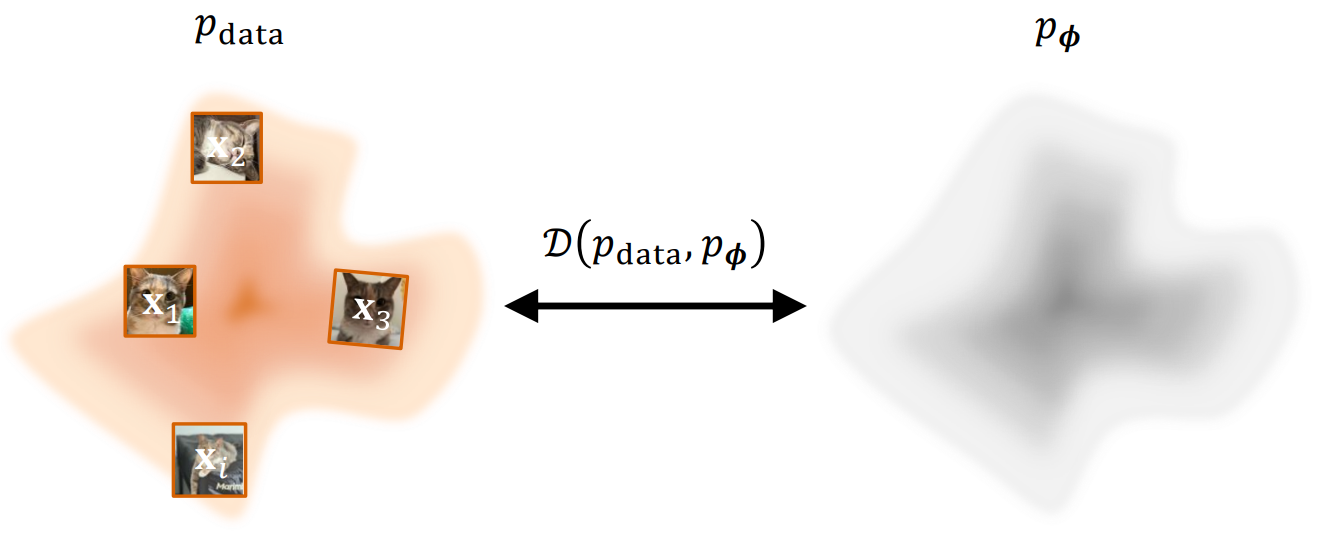
\includegraphics[width=0.8\linewidth]{gfx/dgm/dgm1.png}
    \caption{Visualization of the training of DGMs where we minimize a discrepancy measure between the real and unknown data distribution and the approximated one, using a set of i.i.d. samples.\cite{lai2025principlesdiffusionmodels}}
    \label{fig:dgm1}
\end{figure}

The most common choice is the Kullback-Leibler divergence, defined as 
\begin{equation}
\begin{split}
    \mathcal{D}_{KL}(p_{data}||p_{\theta}) = \int p_{data}(\mathbf{x})\log \frac{p_{data}(\mathbf{x})}{p_{\theta}(\mathbf{x})}d\mathbf{x} = \\ 
    \mathbb{E}_{\mathbf{x}\sim p_{data}}\left[\log p_{data}(\mathbf{x}) - \log p_{\theta}(\mathbf{x})\right],
\end{split}
\end{equation}
where, taking into account only the part that depends 
on the parameter $\theta$, minimizing the KL divergence is equivalent to performing MLE: $$\min_{\theta}\mathcal{D}_{KL}(p_{data}||p_{\theta}) \Longleftrightarrow 
\max_{\theta}\mathbb{E}_{\mathbf{x}\sim p_{data}}\left[\log p_{\theta}(\mathbf{x})\right].$$ In practice, we do not have access to the data distribution, only to 
some i.i.d. samples $\{\mathbf{x}^{(i)}\}_{i=1}^N\sim p_{data}$, which are used to obtain the empirical estimate of the MSE $$\mathcal{L}_{MLE}(\theta) = 
-\frac{1}{N}\sum_{i=1}^N\log p_{\theta}(\mathbf{x}^{(i)}).$$   
There are some challenges in the use of neural networks to parameterize the probability distribution $p_{data}$. We can define a model that produces a real scalar 
$E_{\theta}(\mathbf{x})\in\mathbb{R}$ for input $\mathbf{x}$. To interpret the output as a valid probability density, it has to satisfy the following conditions: 
\begin{itemize}
    \item \textbf{Non-Negativity}: $p_{\theta}(\mathbf{x})\geq 0$ for all $\mathbf{x}$ in the domain. The standard positive function is used to guarantee non-negativity 
    is the exponential function, which produces an unnormalized density $\tilde p_{\theta}(\mathbf{x}) = \exp(E_{\theta}(\mathbf{x}))$.
    \item \textbf{Normalization}: The integral over the entire domain must equal one. To create a valid probability density, we must divide it by its integral over 
    the entire space $$p_{\theta}(\mathbf{x})=\frac{\tilde p_{\theta}(\mathbf{x})}{Z(\theta)},$$ where the denominator is the partition function defined as 
    $$Z(\theta)=\int \tilde p_{\theta}(\mathbf{x'})d\mathbf{x'}.$$ 
\end{itemize}
The partition function introduces a computational challenge in the learning of probabilistic models, especially for high-dimensional problems. This intractability is 
a central problem that motivates the development of many different families of deep generative models, which will be explained in the following chapters. 


%*****************************************
%*****************************************
%*****************************************
%*****************************************
%*****************************************
%************************************************
\chapter{Variational Autoencoders}\label{ch:vaes}
%************************************************

The core initial idea for the understanding of the Variational Autoencoders (VAEs) is the concept of \textbf{Autoencoders} (AEs). 
This are a type of model that contains two elements, the encoder and the decoder. The encoder is a function that maps the input data 
$\mathbf{x}\in\mathbb{R}^d$ to a low-dimensional representation $\mathbf{z}\in\mathbb{R}^k$, which is usually much more smaller than
the input dimension, $k<<d$. This representations live in a space with a more compact and interpretable structure, called the latent space. 
Then, the decoder is a function that maps the latent representation $\mathbf{z}$ back to the input space, trying to reconstruct the 
original data point $\mathbf{x}$. \\
Once we have an autoencoder model trained, a natural question is how to use it as a generative model. One idea is to randomly sample
a point $\mathbf{z}$ from the latent space and then pass it through the decoder to get a synthetic data point $\mathbf{x'}$. This method will 
not produce realistic samples because the latent space is disorganized and irregular. Another option is to encode and image and sample 
neighboring points in the latent space that could generate similar samples, but the reality is that the output are not meaningful samples. This 
shows how poorly structured the latent space is. The aim of VAEs is to transform the latent space of an autoencoder into a well-structured space 
that follows a prior distribution, which allows us to sample from it and generate realistic samples. \\
\\
It is also important to introduce the concept of latent variable models. This type of variables are part of the model 
but are not observed in the data, usually denoted as $\mathbf{z}$, which are the hidden factors of variation. The goal of latent variable models is to 
learn the joint distribution $p_{\theta}(\mathbf{x}, \mathbf{z})$ of the observed data $\mathbf{x}$ and the latent variables $\mathbf{z}$. 
The marginal likelihood, model evidence or marginal distribution over the observed data is given by:
\begin{equation}\label{eq:p_x}
    p_{\theta}(\mathbf{x}) = \int p_{\theta}(\mathbf{x}, \mathbf{z}) d\mathbf{z}.
\end{equation}
When we use neural networks to parameterize the latent variable models we call them \textbf{Deep Latent Variable Models} (DLVMs). 
The simple and most common DLVM is given by the following factorization:
\begin{equation}
    p_{\theta}(\mathbf{x}, \mathbf{z}) = p(\mathbf{z}) p_{\theta}(\mathbf{x} | \mathbf{z}),
\end{equation}
where $p(\mathbf{z})$ is the \textit{prior distribution} over the latent variables and $p_{\theta}(\mathbf{x} | \mathbf{z})$ 
is the likelihood of the data given the latent variables, also called the \textit{generator distribution}. The joint distribution $p_{\theta}(\mathbf{x}, \mathbf{z})$ 
is related through the Bayes' rule to the following posterior distribution:
\begin{equation}
    p_{\theta}(\mathbf{z} | \mathbf{x}) = \frac{p_{\theta}(\mathbf{x} | \mathbf{z}) p(\mathbf{z})}{p_{\theta}(\mathbf{x})},
\end{equation}
where we have an intractability problem due to the marginal likelihood $p_{\theta}(\mathbf{x})$ which is given by an integral over the latent variables (Equation \ref{eq:p_x}). 
To overcome this problem we can use variational inference (VI) which is a technique to approximate the posterior distribution $p_{\theta}(\mathbf{z} | \mathbf{x})$ 
with a simpler distribution $q_{\phi}(\mathbf{z} | \mathbf{x})$ that is parameterized by $\phi$.  \\
\\
This is the main idea behind \textbf{Variational Autoencoders} (VAEs) \cite{kingma2022autoencodingvariationalbayes} which are a type of DLVMs that use VI to learn the latent variable model. It defines a 
parametric inference model $q_{\phi}(\mathbf{z} | \mathbf{x})$, also called an \textit{encoder}, where $\phi$ are the parameters. The idea is to optimize the parameters such that: 
\begin{equation}
    q_{\phi}(\mathbf{z} | \mathbf{x}) \approx p_{\theta}(\mathbf{z} | \mathbf{x}).
\end{equation}
This VAE formulation allows us to transform an autoencoder model with an unstructured latent space into a generative model with a latent space that follows a prior 
distribution, typically a Gaussian distribution $p(\mathbf{z}) = \mathcal{N}(\mathbf{z}; \mathbf{0}, \mathbf{I})$, which is easy to sample from. \\

\begin{figure}
\centering
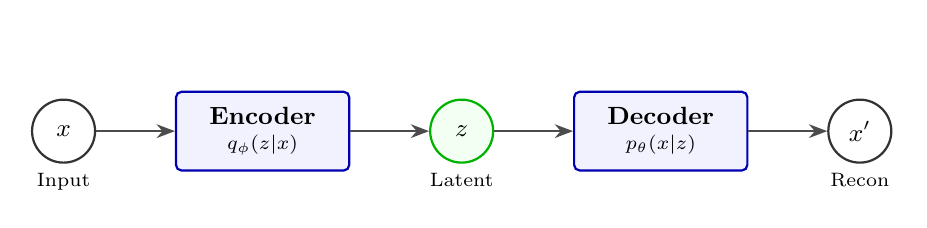
\begin{tikzpicture}[
    >=Stealth,
    node distance=1.0cm, % Very tight spacing
    % Styles for nodes
    block/.style={draw=blue!70!black, fill=blue!5, rectangle, minimum height=1cm, minimum width=2.2cm, align=center, rounded corners=2pt, thick, font=\small\bfseries},
    latentblock/.style={draw=green!70!black, fill=green!5, circle, minimum size=0.8cm, align=center, thick, font=\small},
    io/.style={draw=black!80, fill=white, circle, inner sep=1pt, minimum size=0.8cm, align=center, thick, font=\small}
]

    % Nodes with labels placed below them compactly
    \node (input) [io, label=below:{\scriptsize Input}] {$x$};
    
    \node (encoder) [block, right=of input] {Encoder \\[-0.5ex] \scriptsize $q_{\phi}(z|x)$};
    
    \node (z) [latentblock, right=of encoder, label=below:{\scriptsize Latent}] {$z$};
    
    \node (decoder) [block, right=of z] {Decoder \\[-0.5ex] \scriptsize $p_{\theta}(x|z)$};
    
    \node (output) [io, right=of decoder, label=below:{\scriptsize Recon}] {$x'$};

    % Compact Arrows
    \draw [->, thick, draw=black!70] (input) -- (encoder);
    \draw [->, thick, draw=black!70] (encoder) -- (z);
    \draw [->, thick, draw=black!70] (z) -- (decoder);
    \draw [->, thick, draw=black!70] (decoder) -- (output);

    \path ([yshift=0.8cm]current bounding box.north);

\end{tikzpicture}
\caption{Simplified Variational Autoencoder (VAE) architecture mapping an input $x$ to a latent representation $z$, and decoding it to a reconstruction $x'$.}\label{diag:vae}
\end{figure}


% ******
% Training 
% ******
\section{Training of VAEs} 
For the training of the VAEs we can not directly optimize the marginal likelihood $p_{\theta}(\mathbf{x})$ due to the intractability problem, but we can optimize a lower bound of the marginal likelihood
called the \textbf{Evidence Lower Bound} (ELBO). Let's derive the log-likelihood of the data point $\mathbf{x}$ and see how we can get the ELBO using the Jensen's inequality \cite{Kingma_2019}:
\begin{align}
    \log p_{\theta}(\mathbf{x}) &= \log\int p_{\theta}(\mathbf{x},\mathbf{z})d\mathbf{z} \\ %= \mathbb{E}_{\mathbf{z}\sim q_{\phi}(\mathbf{z} | \mathbf{x})} \left[\log p_{\theta}(\mathbf{x})\right] \\
    &= \log\int q_{\phi}(\mathbf{z}|\mathbf{x})\frac{p_{\theta}(\mathbf{x}, \mathbf{z})}{q_{\phi}(\mathbf{z}|\mathbf{x})}d\mathbf{z} \\
    &= \log \mathbb{E}_{\mathbf{z}\sim q_{\phi}(\mathbf{z}|\mathbf{x})} \left[\frac{p_{\theta}(\mathbf{x},\mathbf{z})}{q_{\phi}(\mathbf{z}|\mathbf{x})}\right] \\
    &\geq \mathbb{E}_{\mathbf{z}\sim q_{\phi}(\mathbf{z}|\mathbf{x})} \left[\log \frac{p_{\theta}(\mathbf{x},\mathbf{z})}{q_{\phi}(\mathbf{z}|\mathbf{x})}\right] \\
    &= \mathbb{E}_{\mathbf{z}\sim q_{\phi}(\mathbf{z}|\mathbf{x})} \left[\log \frac{p_{\theta}(\mathbf{x}|\mathbf{z})p(\mathbf{z})}{q_{\phi}(\mathbf{z}|\mathbf{x})}\right] \\
    &= \mathbb{E}_{\mathbf{z}\sim q_{\phi}(\mathbf{z}|\mathbf{x})} \left[\log \frac{p_{\theta}(\mathbf{x}|\mathbf{z})}{\frac{q_{\phi}(\mathbf{z}|\mathbf{x})}{p(\mathbf{z})}}\right] \\
    &= \mathbb{E}_{\mathbf{z}\sim q_{\phi}(\mathbf{z}|\mathbf{x})} \left[\log p_{\theta}(\mathbf{x}|\mathbf{z}) - \log \frac{q_{\phi}(\mathbf{z}|\mathbf{x})}{p(\mathbf{z})}\right] \\
    &= \underbrace{\mathbb{E}_{\mathbf{z}\sim q_{\phi}(\mathbf{z}|\mathbf{x})} \left[\log p_{\theta}(\mathbf{x}|\mathbf{z})\right]}_{\text{Reconstruction}} - \underbrace{\mathbb{E}_{\mathbf{z}\sim q_{\phi}(\mathbf{z}|\mathbf{x})} \left[\log \frac{q_{\phi}(\mathbf{z}|\mathbf{x})}{p(\mathbf{z})}\right]}_{\text{KL Divergence}}
    %&= \mathbb{E}_{\mathbf{z}\sim q_{\theta}(\mathbf{z}|\mathbf{x})} \left[ \log \left[ \frac{p_{\theta}(\mathbf{x},\mathbf{z})}{q_{\phi}(\mathbf{z} | \mathbf{x})} \frac{q_{\phi}(\mathbf{z}|\mathbf{x})}{p_{\theta}(\mathbf{z}|\mathbf{x})} \right] \right] \\
    %&= \underbrace{\mathbb{E}_{\mathbf{z}\sim q_{\phi}(\mathbf{z}|\mathbf{x})} \left[ \log \frac{p_{\theta}(\mathbf{x}, \mathbf{z})}{q_{\phi}(\mathbf{z}|\mathbf{x})} \right]}_{\text{ELBO Term}} + \underbrace{\mathbb{E}_{\mathbf{z}\sim q_{\phi}(\mathbf{z}|\mathbf{x})} \left[ \log \frac{q_{\phi}(\mathbf{z}|\mathbf{x})}{p_{\theta}(\mathbf{z}|\mathbf{x})} \right]}_{\text{KL Divergence}}.
\end{align}
We can see that for any data point $\mathbf{x}$, the log-likelihood satisfies: 
\begin{align}
    \log p_{\theta}(\mathbf{x}) &\geq \mathcal{L}_{ELBO}(\theta, \phi; \mathbf{x}) \\
    & = \mathbb{E}_{\mathbf{z}\sim q_{\phi}(\mathbf{z}|\mathbf{x})} \left[\log p_{\theta}(\mathbf{x}|\mathbf{z})\right] - \mathcal{D}_{KL}(q_{\phi}(\mathbf{z}|\mathbf{x}) || p(\mathbf{z})).
\end{align}
%The first term is the variational lower bound (ELBO), which can be expressed as:
%\begin{equation}\label{eq:elbos}
%    \mathcal{L}_{ELBO}(\theta, \phi; \mathbf{x}) = \mathbb{E}_{\mathbf{z}\sim q_{\phi}(\mathbf{z}|\mathbf{x})} \left[ \log p_{\theta}(\mathbf{x},\mathbf{z}) - \log q_{\phi}(\mathbf{z}|\mathbf{x}) \right]
%\end{equation}
%The second term is the KL Divergence between the approximate posterior and the true posterior, $D_{KL}(q_{\phi}(\mathbf{z}|\mathbf{x}) || p_{\theta}(\mathbf{z}|\mathbf{x}))$, which is always non-negative. 
%Because of this, eq. (\ref{eq:elbos}) is a lower bound of the log-likelihood of the data point $\mathbf{x}$: 
%\begin{equation}
%    \mathcal{L}_{ELBO}(\theta, \phi; \mathbf{x}) = \log p_{\theta}(\mathbf{x}) - D_{KL}(q_{\phi}(\mathbf{z}|\mathbf{x}) || p_{\theta}(\mathbf{z}|\mathbf{x})) \leq \log p_{\theta}(\mathbf{x}).
%\end{equation}
If we maximize the previous loss with respect to the parameters $\theta$ and $\phi$, we are optimizing: 
\begin{itemize}
    \item \textbf{Reconstruction}: the first term encourage to maximize the likelihood $p_{\theta}(\mathbf{x}|\mathbf{z})$, which corresponds to the reconstruction of the data point $\mathbf{x}$ from the latent variables $\mathbf{z}$. Optimizing this term alone risks memorizing the training data, so we need extra regularization. 
    \item \textbf{Latent KL Regularization}: the second term encourages the encoder distribution $q_{\phi}(\mathbf{z}|\mathbf{x})$ to be close to the prior distribution $p(\mathbf{z})$, which is easy to sample from. 
\end{itemize}
Once we have the definition of the training objective, we can use stochastic gradient descent (SGD) to perform joint optimization w.r.t. all parameters $\theta$ and $\phi$. 
However, we have a problem with the first term of the ELBO because we can not backpropagate through the sampling process of $\mathbf{z}\sim q_{\phi}(\mathbf{z}|\mathbf{x})$, 
as we can see in the left part of Figure \ref{fig:reparameterization}. To solve this problem we can use the \textbf{reparameterization trick} which consists in expressing the sampling 
process as a deterministic function of the parameters and some noise. For example, if we assume that $q_{\phi}(\mathbf{z}|\mathbf{x})$ is a Gaussian distribution with mean $\mu$ and 
variance $\sigma^2$, we can sample from it as follows: 
\begin{equation}
    \mathbf{z} = \mu + \sigma \odot \epsilon, \quad \epsilon \sim \mathcal{N}(0, I).
\end{equation}
This way, we can backpropagate through the deterministic function and optimize the parameters $\phi$ of the encoder. This is shown in the right part of Figure \ref{fig:reparameterization}.

\begin{figure}   
\centering
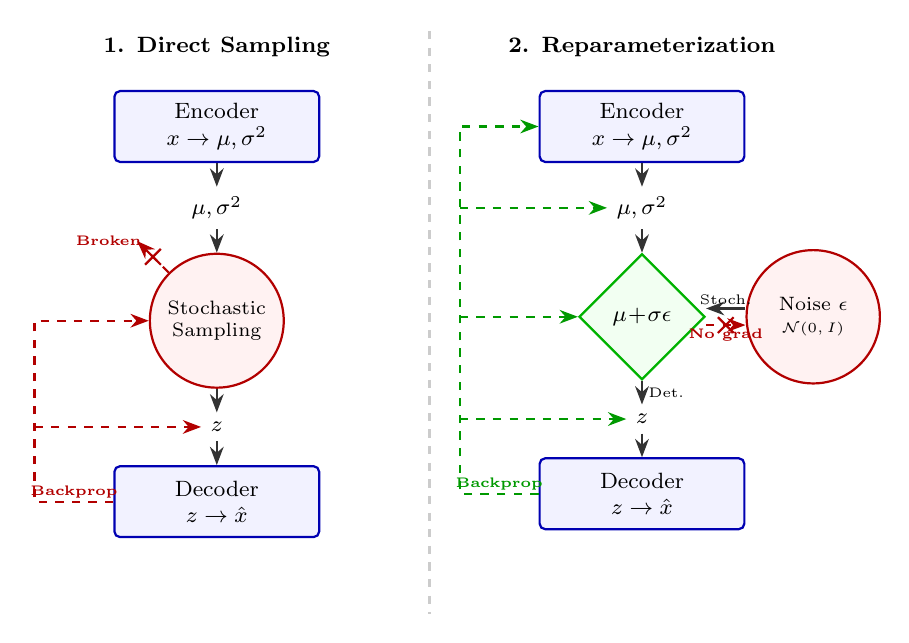
\begin{tikzpicture}[
    >=Stealth,
    node distance=2.0cm, 
    % Scaled-down styles for nodes
    block/.style={draw=blue!70!black, fill=blue!5, rectangle, minimum height=0.9cm, minimum width=2.6cm, align=center, rounded corners=2pt, thick, font=\footnotesize},
    stoch_node/.style={draw=red!70!black, fill=red!5, circle, minimum size=1.5cm, align=center, thick, text width=1.3cm, font=\scriptsize},
    math_op/.style={draw=green!70!black, fill=green!5, diamond, minimum size=1.6cm, align=center, thick, inner sep=0pt, font=\footnotesize},
    io/.style={font=\footnotesize\bfseries},
    % Arrow styles
    forward_arrow/.style={->, thick, draw=black!80},
    grad_fail/.style={->, thick, dashed, draw=red!70!black},
    grad_success/.style={->, thick, dashed, draw=green!60!black}
]

    % ==================== Flow 1: Direct Sampling (LEFT COLUMN) ====================
    % Center of left column is at x=0
    \node (title1) at (0, 0) [font=\footnotesize\bfseries] {1. Direct Sampling};

    \node (encoder1) [block, below=0.3cm of title1] {Encoder\\$x \rightarrow \mu, \sigma^2$};
    \node (mu_sigma1) [below=0.3cm of encoder1, font=\footnotesize] {$\mu, \sigma^2$};
    \node (sampling1) [stoch_node, below=0.3cm of mu_sigma1] {Stochastic\\Sampling};
    \node (z1) [io, below=0.3cm of sampling1] {$z$};
    \node (decoder1) [block, below=0.3cm of z1] {Decoder\\$z \rightarrow \hat{x}$};

    % Forward Arrows (Left)
    \draw [forward_arrow] (encoder1) -- (mu_sigma1);
    \draw [forward_arrow] (mu_sigma1) -- (sampling1);
    \draw [forward_arrow] (sampling1) -- (z1);
    \draw [forward_arrow] (z1) -- (decoder1);

    % Compact Gradient Bus (Routed cleanly on the left)
    \coordinate (grad_bus1) at ($(decoder1.west) + (-1.0cm, 0)$);
    
    \draw [grad_fail] (decoder1.west) -- (grad_bus1) node[midway, above, font=\tiny\bfseries, text=red!70!black, inner sep=1pt] {Backprop} -- (grad_bus1 |- sampling1.west) -- (sampling1.west);
    \draw [grad_fail] (grad_bus1 |- z1.west) -- (z1.west);
    
    % Broken gradient indicator (Fixed alignment and overlap)
    \draw [grad_fail] (sampling1.north west) -- ++(-0.4cm,0.4cm) node[above left, font=\tiny\bfseries, text=red!70!black, inner sep=1pt, xshift=0.1cm, yshift=-0.1cm] {Broken};
    \coordinate (break_pt1) at ($(sampling1.north west) + (-0.2cm, 0.2cm)$);
    \draw [thick, red!70!black] ($(break_pt1)+(-0.1cm,-0.1cm)$) -- +(0.2cm,0.2cm);
    \draw [thick, red!70!black] ($(break_pt1)+(-0.1cm,0.1cm)$) -- +(0.2cm,-0.2cm);


    % ==================== Flow 2: Reparameterization (RIGHT COLUMN) ====================
    % Center of right column is slightly wider to give the green gradient bus room
    \node (title2) at (5.4cm, 0) [font=\footnotesize\bfseries] {2. Reparameterization};

    \node (encoder2) [block, below=0.3cm of title2] {Encoder\\$x \rightarrow \mu, \sigma^2$};
    \node (mu_sigma2) [below=0.3cm of encoder2, font=\footnotesize] {$\mu, \sigma^2$};
    
    \node (math_op2) [math_op, below=0.3cm of mu_sigma2] {$ \mu \!+\! \sigma \epsilon $};
    
    % Noise Node
    \node (epsilon2) [stoch_node, right=0.5cm of math_op2] {Noise $\epsilon$\\ \tiny $\mathcal{N}(0, I)$};

    \node (z2) [io, below=0.3cm of math_op2] {$z$};
    \node (decoder2) [block, below=0.3cm of z2] {Decoder\\$z \rightarrow \hat{x}$};

    % Forward Arrows (Right)
    \draw [forward_arrow] (encoder2) -- (mu_sigma2);
    \draw [forward_arrow] (mu_sigma2) -- (math_op2);
    
    % FIXED: Split the bidirectional arrows between Diamond and Noise so they don't overlap
    % 1. Forward stochastic path (Shifted slightly up)
    \draw [forward_arrow] ([yshift=3pt]epsilon2.west) -- ([yshift=3pt]math_op2.east) node[midway, above, font=\tiny, inner sep=1pt] {Stoch.};
    
    % FIXED: "Det." text moved slightly right so it doesn't clip the diamond
    \draw [forward_arrow] (math_op2.south) -- (z2.north) node[midway, right, font=\tiny, inner sep=2pt] {Det.};
    \draw [forward_arrow] (z2) -- (decoder2);

    % Compact Gradient Bus (Right) - Now sitting comfortably on the left of the blocks
    \coordinate (grad_bus2) at ($(decoder2.west) + (-1.0cm, 0)$);
    \coordinate (grad_bus2_top) at ($(encoder2.west) + (-1.0cm, 0)$);
    
    \draw [grad_success] (decoder2.west) -- (grad_bus2) node[midway, above, font=\tiny\bfseries, text=green!60!black, inner sep=1pt] {Backprop} -- (grad_bus2_top) -- (encoder2.west);
    
    % Connecting intermediate nodes to success bus
    \draw [grad_success] (grad_bus2 |- z2.west) -- (z2.west);
    \draw [grad_success] (grad_bus2 |- math_op2.west) -- (math_op2.west);
    \draw [grad_success] (grad_bus2 |- mu_sigma2.west) -- (mu_sigma2.west);
    
    % FIXED: Backward gradient fail path (Shifted slightly down to separate from forward path)
    \draw [grad_fail] ([yshift=-3pt]math_op2.east) -- ([yshift=-3pt]epsilon2.west) node[midway, below, font=\tiny\bfseries, text=red!70!black, inner sep=1pt] {No grad};
    
    % Cross mark correctly positioned directly on the shifted "No grad" line
    \coordinate (cross_pt) at ($([yshift=-3pt]math_op2.east)!0.5!([yshift=-3pt]epsilon2.west)$);
    \draw [thick, red!70!black] ($(cross_pt)+(-0.1cm,-0.1cm)$) -- +(0.2cm,0.2cm);
    \draw [thick, red!70!black] ($(cross_pt)+(-0.1cm,0.1cm)$) -- +(0.2cm,-0.2cm);

    % Divider line perfectly centered between the two column bounding boxes
    \draw [dashed, draw=gray!40, thick] (2.7cm, 0.2cm) -- (2.7cm, -7.2cm);

\end{tikzpicture}
\caption{Reparameterization Trick in VAEs}
\label{fig:reparameterization}
\end{figure}


% ******
% Gaussian VAEs 
% ******
\section{Gaussian VAEs}
The common choice for both the encoder and the decoder distributions in VAEs is the Gaussian distribution. This is because it allows us to use the reparameterization trick and 
also because it has a closed-form expression for the KL divergence. \\
The \textbf{encoder} $q_{\phi}(\mathbf{z}|\mathbf{x})$ is modelled as a Gaussian distribution defined as:
\begin{equation}
    q_{\phi}(\mathbf{z}|\mathbf{x}) = \mathcal{N} \left(\mathbf{z}; \mu_{\phi}(\mathbf{x}), \text{diag}(\sigma^2_{\phi}(\mathbf{x})) \right),
\end{equation}
where $\mu_{\phi}(\mathbf{x})$ and $\sigma^2_{\phi}(\mathbf{x})$ are the mean and variance of the Gaussian distribution, which are parameterized by a neural network with parameters $\phi$. \\
The \textbf{decoder} $p_{\theta}(\mathbf{x}|\mathbf{z})$ is also modelled as a Gaussian distribution defined as:
\begin{equation}
    p_{\theta}(\mathbf{x}|\mathbf{z}) = \mathcal{N} \left(\mathbf{x}; \mu_{\theta}(\mathbf{z}), \sigma^2\mathbf{I} \right),
\end{equation}
where $\mu_{\theta}(\mathbf{z})$ is the mean of the Gaussian distribution, which is parameterized by a neural network with parameters $\theta$, and $\sigma^2\mathbf{I}$ is the covariance matrix, 
which is usually fixed to be a diagonal matrix with constant variance. \\ 
\\
Under this Gaussian assumption, we can obtain a closed-form expression for the ELBO loss function. The reconstruction term can be expressed as:
\begin{equation}
    \mathbb{E}_{\mathbf{z}\sim q_{\phi}(\mathbf{z}|\mathbf{x})} \left[\log p_{\theta}(\mathbf{x}|\mathbf{z})\right] = -\frac{1}{2\sigma^2} \mathbb{E}_{\mathbf{z}\sim q_{\phi}(\mathbf{z}|\mathbf{x})} \left[||\mathbf{x} - \mu_{\theta}(\mathbf{z})||^2\right] + C,
\end{equation}
where $C$ is a constant that does not depend on the parameters. The KL divergence term can be expressed as:
\begin{equation}
    \mathcal{D}_{KL}(q_{\phi}(\mathbf{z}|\mathbf{x}) || p(\mathbf{z})) = \frac{1}{2} \sum_{i=1}^k \left( \sigma^2_{\phi,i}(\mathbf{x}) + \mu^2_{\phi,i}(\mathbf{x}) - 1 - \log \sigma^2_{\phi,i}(\mathbf{x}) \right),
\end{equation}
where $k$ is the dimension of the latent space. Therefore, the ELBO loss function can be expressed as:
\begin{align}
    \mathcal{L}_{ELBO}(\theta, \phi; \mathbf{x}) &= -\frac{1}{2\sigma^2} \mathbb{E}_{\mathbf{z}\sim q_{\phi}(\mathbf{z}|\mathbf{x})} \left[||\mathbf{x} - \mu_{\theta}(\mathbf{z})||^2\right] \\ 
    &- \frac{1}{2} \sum_{i=1}^k \left( \sigma^2_{\phi,i}(\mathbf{x}) + \mu^2_{\phi,i}(\mathbf{x}) - 1 - \log \sigma^2_{\phi,i}(\mathbf{x}) \right) + C.
\end{align} 
Despite their mathematical elegance and continuous latent spaces, standard Gaussian Variational Autoencoders notoriously suffer from generating blurry images. 
This limitation fundamentally stems from the VAE objective function and its underlying statistical assumptions. The problem can be attributed to four primary factors:
\begin{itemize}
    \item \textbf{MSE Loss}: In a standard Gaussian VAE with a fixed variance $\sigma^2 \mathbf{I}$, maximizing the likelihood $p_\theta(\mathbf{x}|\mathbf{z})$ is mathematically equivalent to 
    minimizing the $\mathcal{L}_2$ distance between the input $\mathbf{x}$ and the reconstruction $\hat{\mathbf{x}}$:
    \begin{equation}
        \log p_\theta(\mathbf{x}|\mathbf{z}) \propto -||\mathbf{x} - \mu_\theta(\mathbf{z})||^2_2
        \label{eq:vae_mse}
    \end{equation}
    The $\mathcal{L}_2$ loss heavily penalizes large pixel-wise deviations. When the model is uncertain about the exact location of high-frequency details (such as sharp edges), it outputs the statistical 
    mean of all plausible variations to minimize the overall penalty. This phenomenon, known as \textit{mode averaging}, results in safe, blurry predictions rather than rendering sharp, distinct features.
    \item \textbf{Information Bottleneck}: The ELBO includes a regularization term that minimizes the KL divergence between the approximate posterior and the prior:
    \begin{equation}
        \mathcal{D}_{\text{KL}}(q_\phi(\mathbf{z}|\mathbf{x}) \parallel p(\mathbf{z}))
        \label{eq:vae_kl}
    \end{equation}
    This term acts as an information bottleneck, forcing the encoded latent representations to closely match the simple prior, typically $\mathcal{N}(\mathbf{0}, \mathbf{I})$. Consequently, the encoder 
    discards complex, high-frequency spatial features that are difficult to compress, prioritizing global structures and low-frequency components instead.
    \item \textbf{Posterior Collapse}: Furthermore, consistent with findings in \cite{bowman2016generatingsentencescontinuousspace} and \cite{sonderby2016howtrain}, stochastic optimization using the unmodified lower bound objective frequently 
    gets stuck in an undesirable stable equilibrium. At the onset of training, the reconstruction likelihood term $\log p_\theta(\mathbf{x}|\mathbf{z})$ is relatively weak. Consequently, an initially 
    attractive state for the network is to aggressively minimize the latent cost, driving the approximate posterior to match the prior, $q_\phi(\mathbf{z}|\mathbf{x}) \approx p(\mathbf{z})$. This results 
    in a stable equilibrium---often termed \textit{posterior collapse}---from which the model struggles to escape, yielding uninformative latent representations and contributing to poor generation quality. 
    To mitigate this, a common solution proposed in \cite{bowman2016generatingsentencescontinuousspace, sonderby2016howtrain} is to implement an optimization schedule (KL annealing) where the weight of the latent cost 
    $\mathcal{D}_{\text{KL}}(q_\phi(\mathbf{z}|\mathbf{x}) \parallel p(\mathbf{z}))$ is slowly annealed from 0 to 1 over multiple epochs.
\end{itemize}


% ******
% DDPMs 
% ******
\section{Denoising Diffusion Probabilistic Models}
One important technique developed to enhance the performance of VAEs and overcome the main limitations was \textbf{Hierarchical Variational Autoencoders} (HVAEs) \cite{vahdat2021nvaedeephierarchicalvariational} which are a type of VAE that uses a hierarchical 
structure in the latent space. This hierarchical structure allows the model to capture more complex and high-frequency details in the data, which can help to reduce the blurriness of the generated images. A visualization of the 
architecture of HVAEs is shown in Figure \ref{fig:hvvae}. In this architecture, we have $L$ layers of latent variables $\mathbf{z}_1, \mathbf{z}_2, \dots, \mathbf{z}_L$, where each layer captures different levels of abstraction. \\
In this setup, we can define the following factorization of the joint distribution: 
\begin{figure}   
\centering
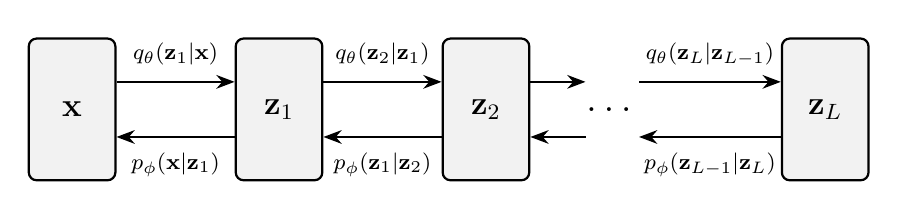
\begin{tikzpicture}[
    % Tighter styles for narrower fit
    block/.style={
        draw,
        thick,
        rectangle,
        rounded corners=1mm,
        minimum width=1.1cm,
        minimum height=1.8cm,
        fill=black!5,
        font=\large,
        align=center
    },
    arr/.style={->, thick, >=Stealth},
    revarr/.style={<-, thick, >=Stealth},
    % Added a label style to make the math font slightly smaller and reduce padding
    lbl/.style={midway, font=\footnotesize, inner sep=5.5pt} 
]

    % --- Nodes ---
    \node[block] (x) {$\mathbf{x}$};
    \node[block, right=1.5cm of x] (z1) {$\mathbf{z}_1$};
    \node[block, right=1.5cm of z1] (z2) {$\mathbf{z}_2$};
    
    % Reduced the space around the ellipsis
    \node[right=0.7cm of z2, font=\Large, inner xsep=0mm] (dots) {$\dots$};
    
    \node[block, right=1.8cm of dots] (zl) {$\mathbf{z}_L$};

    % --- Edges ---
    % Brought the arrows slightly closer together (yshift=3.5mm instead of 5mm)
    
    % Connections between x and z1
    \draw[arr]    ([yshift=3.5mm]x.east) -- ([yshift=3.5mm]z1.west)
        node[lbl, above] {$q_\theta(\mathbf{z}_1|\mathbf{x})$};
    \draw[revarr] ([yshift=-3.5mm]x.east) -- ([yshift=-3.5mm]z1.west)
        node[lbl, below] {$p_\phi(\mathbf{x}|\mathbf{z}_1)$};

    % Connections between z1 and z2
    \draw[arr]    ([yshift=3.5mm]z1.east) -- ([yshift=3.5mm]z2.west)
        node[lbl, above] {$q_\theta(\mathbf{z}_2|\mathbf{z}_1)$};
    \draw[revarr] ([yshift=-3.5mm]z1.east) -- ([yshift=-3.5mm]z2.west)
        node[lbl, below] {$p_\phi(\mathbf{z}_1|\mathbf{z}_2)$};

    % Connections entering the ellipsis from z2
    \draw[arr]    ([yshift=3.5mm]z2.east) -- ([yshift=3.5mm]dots.west);
    \draw[revarr] ([yshift=-3.5mm]z2.east) -- ([yshift=-3.5mm]dots.west);

    % Connections leaving the ellipsis to zL
    \draw[arr]    ([yshift=3.5mm]dots.east) -- ([yshift=3.5mm]zl.west)
        node[lbl, above] {$q_\theta(\mathbf{z}_L|\mathbf{z}_{L-1})$};
    \draw[revarr] ([yshift=-3.5mm]dots.east) -- ([yshift=-3.5mm]zl.west)
        node[lbl, below] {$p_\phi(\mathbf{z}_{L-1}|\mathbf{z}_L)$};

\end{tikzpicture}
\caption{Hierarchical VAE architecture with $L$ layers of latent variables. Each layer captures different levels of abstraction, allowing for richer representations and improved generation quality.}
\label{fig:hvvae}
\end{figure}
\begin{equation}
    p_{\theta}(\mathbf{x},\mathbf{z}_{1:L}) = p_{\theta}(\mathbf{x}|\mathbf{z}_1)\prod_{i=2}^{L} p_{\theta}(\mathbf{z}_{i-1}|\mathbf{z}_i)p(\mathbf{z}_L),
\end{equation}
and the marginal distribution of the data point $\mathbf{x}$ can be expressed as:
\begin{equation}
    p_{\theta}(\mathbf{x}) = \int p_{\theta}(\mathbf{x},\mathbf{z}_{1:L})d\mathbf{z}_{1:L},
\end{equation}
where the generation is performed progressively from the latent variable $\mathbf{z}_L$, which follows the prio distribution $p(\mathbf{z}_L)$, to the data point $\mathbf{x}$, which is generated from the latent variable $\mathbf{z}_1$.
The inference model can be defined as: 
\begin{equation}
    q_{\phi}(\mathbf{z}_{1:L}|\mathbf{x}) = q_{\phi}(\mathbf{z}_1|\mathbf{x})\prod_{i=2}^{L} q_{\phi}(\mathbf{z}_i|\mathbf{z}_{i-1}),
\end{equation}
where the inference is performed progressively from the data point $\mathbf{x}$ to the latent variable $\mathbf{z}_L$. \\
The ELBO loss is very similar to the one of the standard VAE, but we have to consider all the layers of latent variables:
\begin{align}
    \mathcal{L}_{ELBO}(\theta, \phi; \mathbf{x}) &= \mathbb{E}_{\mathbf{z}_{1:L}\sim q_{\phi}(\mathbf{z}_{1:L}|\mathbf{x})} \left[\log \frac{p_{\theta}(\mathbf{x},\mathbf{z}_{1:L})}{q_{\phi}(\mathbf{z}_{1:L}|\mathbf{x})} \right],
\end{align}
which can also be decomposed into the reconstruction term and the KL divergence term. \\
\\
This method of deep, stacked layers revolutionized the field of generative modeling and is the basis for many state-of-the-art models. The training of HVAEs present several challenges because the encoder 
and decoder must be trained jointly and learning becomes unstable. A clever twist to solve the main problems and maintain the hierarchical structure is the \textbf{Denoising Diffusion Probabilistic Models} (DDPMs)
\cite{sohldickstein2015deepunsupervisedlearningusing, ho2020denoisingdiffusionprobabilisticmodels}, the next step in generative modeling, that can be defined with the following stochastic processes. \\
\\
\textbf{Forward Pass}. This is a fixed encoder (not learnable) that progressively adds noise to the data point $\mathbf{x}$ via a transition 
kernel $p(\mathbf{x}_t|\mathbf{x}_{t-1})$ until we get pure noise $\mathbf{x}_T \sim \mathcal{N}(\mathbf{0}, \mathbf{I})$. The fixed Gaussian transition kernel is defined as:
\begin{equation}\label{eq:forward_kernel}
    p(\mathbf{x}_t|\mathbf{x}_{t-1}) = \mathcal{N}(\mathbf{x}_t; \sqrt{1-\beta_t}\mathbf{x}_{t-1}, \beta_t\mathbf{I}),
\end{equation} 
where $\mathbf{x}_0\sim p_{data}$, $\mathbf{x}_T \sim \mathcal{N}(\mathbf{0}, \mathbf{I})$ and the sequence $\{\beta_t\}_{t=1}^T\in(0,1)$ is the 
noise schedule, which controls the amount of noise added at each step, as we can clearly see in the following formulation: 
\begin{equation}\label{eq:forward_sample}
    \mathbf{x}_t = \sqrt{\alpha_t} \mathbf{x}_{t-1} + \sqrt{1-\alpha_t} \epsilon, \quad \epsilon \sim \mathcal{N}(\mathbf{0}, \mathbf{I}),
\end{equation}
where $\alpha_t = 1-\beta_t$. Another important formulation of the forward pass can be achieve by recursively applying the transition kernel (Equation \ref{eq:forward_kernel}), 
where we achieve a closed-form expression for the distribution of noisy samples at step $t$ given the original data:
\begin{equation}
    p(\mathbf{x}_t|\mathbf{x}_0) = \mathcal{N}(\mathbf{x}_t; \sqrt{\bar{\alpha}_t}\mathbf{x}_0, (1-\bar{\alpha}_t)\mathbf{I}),
\end{equation}
where $\bar{\alpha}_t = \prod_{s=1}^T \alpha_s$. This formulation is very useful because it allows us to sample from the forward process at any 
time step $t$ without having to recursively apply the transition kernel $t$ times. We can also define the sampling of $\mathbf{x}_t$ as in Equation \ref{eq:forward_sample} as follows:
\begin{equation}\label{eq:forward_sample2}
    \mathbf{x}_t = \sqrt{\bar\alpha_t} \mathbf{x}_0 + \sqrt{1-\bar{\alpha}_t} \epsilon, \quad \epsilon \sim \mathcal{N}(\mathbf{0}, \mathbf{I}).
\end{equation}
\\
\textbf{Reverse Pass}: This is the decoder, where a neural network is trained to reverse the noising process by learning the parameterized 
distribution $p_{\theta}(\mathbf{x}_{t-1}|\mathbf{x}_t)$. If we start from a pure noise sample, we can iteratively apply the reverse process 
to generate a data point $\mathbf{x}_0$ that resembles the training data, following a Markov chain. The training goal is to approximate the unknown reverse transition 
kernel $p(\mathbf{x}_{t-1}|\mathbf{x}_t)$ with a learnable parametric model $p_{\theta}(\mathbf{x}_{t-1}|\mathbf{x}_t)$, using the KL divergence 
as the training objective: 
\begin{equation}\label{eq:kl_reverse}
    \mathbb{E}_{\mathbf{x}_t \sim p_t} \left[ \mathcal{D}_{KL}(p(\mathbf{x}_{t-1}|\mathbf{x}_t) || p_{\theta}(\mathbf{x}_{t-1}|\mathbf{x}_t)) \right].
\end{equation}
We can express the unknown reverse transition kernel $p(\mathbf{x}_{t-1}|\mathbf{x}_t)$ in terms of the forward process using Bayes' rule:
\begin{equation}
    p(\mathbf{x}_{t-1}|\mathbf{x}_t) = \frac{p(\mathbf{x}_t|\mathbf{x}_{t-1}) p_{t-1}(\mathbf{x}_{t-1})}{p_t(\mathbf{x}_t)},
\end{equation}
where the marginal distribution $p_t(\mathbf{x}_t)$ can be expressed as:
\begin{equation}
    p_t(\mathbf{x}_t) = \int p(\mathbf{x}_t|\mathbf{x}_0) p_{data}(\mathbf{x}_0) d\mathbf{x}_0.
\end{equation}
Since $p_{data}$ is unknown, we can not compute the marginal distribution $p_t(\mathbf{x}_t)$ thus the computation of the target distribution 
$p(\mathbf{x}_{t-1}|\mathbf{x}_t)$ is intractable. A trick to solve this problem is to condition the reverse transition kernel on the original data 
point $\mathbf{x}_0$. Now we can define the target distribution as follows:
\begin{equation}
    p(\mathbf{x}_{t-1}|\mathbf{x}_t, \mathbf{x}_0) = \frac{p(\mathbf{x}_t|\mathbf{x}_{t-1}) p_{t-1}(\mathbf{x}_{t-1}|\mathbf{x}_0)}{p_t(\mathbf{x}_t|\mathbf{x}_0)},
\end{equation}
which allows us to have a tractable expression and to derive a tractable objective equivalent to the previous intractable KL divergence in Equation \ref{eq:kl_reverse}. 
As a result, $p(\mathbf{x}_{t-1}|\mathbf{x}_t, \mathbf{x}_0)$ is a Gaussian distribution with mean and variance that can be computed in closed-form: 
\begin{equation}
    p(\mathbf{x}_{t-1}|\mathbf{x}_t, \mathbf{x}_0) = \mathcal{N}(\mathbf{x}_{t-1}; \tilde{\mu}_t(\mathbf{x}_t, \mathbf{x}_0, t), \sigma^2(t)\mathbf{I}),
\end{equation}
where 
\begin{equation}\label{eq:tilde_mean}
    \tilde{\mu}_t(\mathbf{x}_t, \mathbf{x}_0, t) = \frac{\sqrt{\bar{\alpha}_{t-1}}\beta_t}{1-\bar{\alpha}_t}\mathbf{x}_0 + \frac{(1-\bar{\alpha}_{t-1})\sqrt{\alpha}_t}{1-\bar{\alpha}_t}\mathbf{x}_t, \quad \sigma^2(t) = \frac{1-\bar{\alpha}_{t-1}}{1-\bar{\alpha}_t}\beta_t.
\end{equation}
Finally, DDPM assumes that each reverse transition kernel $p_{\theta}(\mathbf{x}_{t-1}|\mathbf{x}_t)$ is a Gaussian distribution with mean $\mu_{\theta}(\mathbf{x}_t, t)$ 
and variance $\sigma^2(t)\mathbf{I}$, where the variance is fixed and the mean is parameterized by a neural network with parameters $\theta$. It can be defined as 
\begin{equation}
    p_{\theta}(\mathbf{x}_{t-1}|\mathbf{x}_t) = \mathcal{N}(\mathbf{x}_{t-1}; \mu_{\theta}(\mathbf{x}_t, t), \sigma^2(t)\mathbf{I}).
\end{equation}
Using the previous conditional derivation of the unknown reverse transition kernel, we can define a closed-form expression for the KL divergence training loss:
\begin{equation}\label{eq:loss_ddpm}
    \mathcal{L}(\mathbf{x}_0;\theta) = \mathbb{E}_{t, \mathbf{x}_0} \left[\frac{1}{2\sigma^2(t)} ||\mu_{\theta}(\mathbf{x}_t, t) - \tilde{\mu}_t(\mathbf{x}_t, \mathbf{x}_0, t)||^2 + C \right].
\end{equation}
where $C$ is a constant that does not depend on the parameters. This loss can be interpreted as a weighted $\mathcal{L}_2$ loss between the predicted mean 
$\mu_{\theta}(\mathbf{x}_t, t)$ and the true mean $\tilde{\mu}_t(\mathbf{x}_t, \mathbf{x}_0, t)$ of the reverse transition kernel. \\
In practice, we do not use the loss of Equation \ref{eq:loss_ddpm} directly. If we combine the definition of the true mean $\tilde{\mu}_t(\mathbf{x}_t, \mathbf{x}_0, t)$ in Equation 
\ref{eq:tilde_mean} with Equation \ref{eq:forward_sample2}, we can obtain two different parameterizations of the mean that can be used to derive two different but equivalent training 
losses that are easier to optimize. 
\begin{itemize}
    \item $\epsilon$-Prediction. From Equation \ref{eq:forward_sample2} we obtain $\mathbf{x}_0 = \frac{1}{\sqrt{\bar{\alpha}_t}}(\mathbf{x}_t - \sqrt{1-\bar{\alpha}_t}\epsilon)$ and we can 
    substitute this expression in the definition of the true mean $\tilde{\mu}_t(\mathbf{x}_t, \mathbf{x}_0, t)$ to obtain the following expression:
    \begin{equation}
        \tilde{\mu}_t(\mathbf{x}_t, \mathbf{x}_0, t) = \frac{1}{\sqrt{\alpha}_t} \left( \mathbf{x}_t - \frac{\beta_t}{\sqrt{1-\bar{\alpha}_t}} \epsilon \right),
    \end{equation}
    which can also be applied to parameterized mean using now a neural network that predicts the noise $\epsilon_{\theta}(\mathbf{x}_t, t)$ instead of the mean $\mu_{\theta}(\mathbf{x}_t, t)$:
    \begin{equation}
    \mu_{\theta}(\mathbf{x}_t, t) = \frac{1}{\sqrt{\alpha}_t} \left( \mathbf{x}_t - \frac{\beta_t}{\sqrt{1-\bar{\alpha}_t}} \epsilon_{\theta}(\mathbf{x}_t, t) \right).
    \end{equation}
    We can define a new loss function based on the noise prediction as follows:
    \begin{equation}
        \mathcal{L}(\mathbf{x}_0;\theta) = \mathbb{E}_{t, \mathbf{x}_0, \epsilon} \left[\frac{\beta_t^2}{2\sigma^2(t)\alpha_t(1-\bar{\alpha}_t)} ||\epsilon_{\theta}(\mathbf{x}_t, t) - \epsilon||^2 \right],
    \end{equation}
    where a simple version of this loss, where the weighting factor is removed, is commonly used in practice for the good performance and stability of the training process found in \cite{ho2020denoisingdiffusionprobabilisticmodels}.
    The final loss can be expressed as: 
    \begin{equation}
        \mathcal{L}(\mathbf{x}_0;\theta) = \mathbb{E}_{t, \mathbf{x}_0, \epsilon} \left[||\epsilon_{\theta}(\mathbf{x}_t, t) - \epsilon||^2 \right].
    \end{equation}
    \item $\mathbf{x}_0$-Prediction: With the definition of the true mean $\tilde{\mu}_t(\mathbf{x}_t, \mathbf{x}_0, t)$ (Equation \ref{eq:tilde_mean}) we can obtain 
    a new parameterization of the mean by using a neural network that predicts the original data point $\mathbf{x}_0$ instead of the mean $\mu_{\theta}(\mathbf{x}_t, t)$:
    \begin{equation}
        \mu_{\theta}(\mathbf{x}_t, t) = \frac{\sqrt{\bar{\alpha}_{t-1}}\beta_t}{1-\bar{\alpha}_t}\mathbf{x}_{\theta}(\mathbf{x}_t, t) + \frac{(1-\bar{\alpha}_{t-1})\sqrt{\alpha}_t}{1-\bar{\alpha}_t}\mathbf{x}_t,
    \end{equation}
    which, as in the previous case, can be used to derive a new loss function based on the original data point prediction as follows:
    \begin{equation}
        \mathcal{L}(\mathbf{x}_0;\theta) = \mathbb{E}_{t, \mathbf{x}_0, \epsilon} \left[\omega_t||\mathbf{x}_{\theta}(\mathbf{x}_t, t) - \mathbf{x}_0||^2 \right].
    \end{equation}
    where $\omega_t$ is a weighting factor that depends on the noise schedule and the variance of the reverse transition kernel, which can be ignored in practice. 
\end{itemize}








\newpage
\begin{summarybox}[label={box:latent_math}]{VAEs and DDPMs}
    This box summarizes the main mathematical equations of VAEs and DDPMs:

    \medskip
    \textbf{1. Training Objective of VAEs:}
    \begin{equation}
        \mathcal{L}_{ELBO}(\theta, \phi; \mathbf{x}) = \mathbb{E}_{\mathbf{z}\sim q_{\phi}(\mathbf{z}|\mathbf{x})} \left[\log p_{\theta}(\mathbf{x}|\mathbf{z})\right] - \mathcal{D}_{KL}(q_{\phi}(\mathbf{z}|\mathbf{x}) || p(\mathbf{z})).
    \end{equation}

    \medskip
    \textbf{2. Training Objective of Gaussian VAEs:}
    \begin{align}
        &\mathcal{L}_{ELBO}(\theta, \phi; \mathbf{x}) = -\frac{1}{2\sigma^2} \mathbb{E}_{\mathbf{z}\sim q_{\phi}(\mathbf{z}|\mathbf{x})} \left[||\mathbf{x} - \mu_{\theta}(\mathbf{z})||^2\right] \\ 
        &- \frac{1}{2} \sum_{i=1}^k \left( \sigma^2_{\phi,i}(\mathbf{x}) + \mu^2_{\phi,i}(\mathbf{x}) - 1 - \log \sigma^2_{\phi,i}(\mathbf{x}) \right) + C.
    \end{align} 

    \medskip
    \textbf{3. Forward Pass in DDPMs:}
    \begin{align}
        & p(\mathbf{x}_t|\mathbf{x}_{t-1}) = \mathcal{N}(\mathbf{x}_t; \sqrt{1-\beta_t}\mathbf{x}_{t-1}, \beta_t\mathbf{I}) \\
        & p(\mathbf{x}_t|\mathbf{x}_0) = \mathcal{N}(\mathbf{x}_t; \sqrt{\bar{\alpha}_t}\mathbf{x}_0, (1-\bar{\alpha}_t)\mathbf{I})
    \end{align} 

    \medskip
    \textbf{4. $\epsilon$-Prediction loss in DDPMs:}
    \begin{equation}
        \mathcal{L}(\theta) = \mathbb{E}_{t, \mathbf{x}_0, \epsilon} \left[||\epsilon_{\theta}(\mathbf{x}_t, t) - \epsilon||^2 \right].
    \end{equation} 

    \medskip
    \textbf{5. $\mathbf{x}_0$-Prediction loss in DDPMs:}
    \begin{equation}
        \mathcal{L}(\theta) = \mathbb{E}_{t, \mathbf{x}_0, \epsilon} \left[\omega_t||\mathbf{x}_{\theta}(\mathbf{x}_t, t) - \mathbf{x}_0||^2 \right].
    \end{equation} 
    
    %\vsub
    %{\small \color{boxaccent}\textbf{Note:} Ensure latent dimensions $z_i$ and $z_j$ maintain near-zero mutual information to preserve explainability.}
\end{summarybox} 


%*****************************************
%*****************************************
%*****************************************
%*****************************************
%***************************************** 
%%************************************************
\chapter{Diffusion Models}\label{ch:diffusion}
%************************************************

Diffusion Models.


%*****************************************
%*****************************************
%*****************************************
%*****************************************
%*****************************************
%************************************************
\chapter{Energy-Based Models}\label{ch:ebms}
%************************************************

Energy-Based Models (EBMs) \cite{lecun2006tutorial} are a general class of models that capture dependencies by associating 
a scalar energy value to each configuration of variables, acting as a measure of compatibility.
\begin{itemize}
    \item \textbf{Training}: The general principle is to find an energy function that associates low energies to correct 
    (observed) configurations of variables, and higher energies to incorrect (unobserved) configurations.
    \item \textbf{Inference}: Making a decision consists of setting the values of observed variables and finding values 
    for the missing variables that minimize the energy, i.e., finding the values most compatible with the observation. 
    In the simplest scenario with two variables $X$ and $Y$, where the first is observed, the model will produce an 
    answer $Y^*$ that is the most compatible with $X$. This procedure is formally defined as:
    \begin{equation}
        Y^*=\text{argmin}_{Y\in \mathcal{Y}}E(X,Y).
    \end{equation} 
    When the size of the set $\mathcal{Y}$ is small, we can simply compute the energy for all possible values and pick 
    the smallest. However, we typically deal with complex, high-dimensional spaces where exhaustive search is impractical. 
    The solution is to apply an inference procedure to obtain an approximate result, which may or may not be the global 
    minimum of the energy function. For example, for a continuous variable $Y$ and a smooth, well-behaved energy function, 
    gradient-based optimization algorithms can be utilized.
\end{itemize}
The scenario described above covers prediction, classification, and decision-making, answering the question: "Which value 
of Y is most compatible with this X?". One advantage of these models is that we can use energy-based models to answer different 
types of questions. (I) Ranking, "Is Y1 or Y2 more compatible with this X?"; (II) Detection, "Is this value of Y compatible 
with X?"; and (III) Conditional density estimation, "What is the conditional probability distribution over $\mathcal{Y}$ 
given X?".  \\
\\
In deterministic settings, we only require the system to assign the lowest energy to the correct value, allowing us to ignore 
the absolute scale of the remaining large energies. However, if these outputs need to be rigorously compared, combined, or 
utilized to quantify uncertainty, uncalibrated energies are insufficient. We can calibrate energies by transforming them 
into a normalized probability distribution using the Gibbs distribution:
\begin{equation}
    p_{\theta}(\mathbf{x}) = \frac{e^{-E_{\theta}(\mathbf{x})}}{Z_{\theta}}, \qquad Z_{\theta}=\int_{\mathbf{x}\in\mathcal{X}} e^{-E_{\theta}(\mathbf{x})}d\mathbf{x}
\end{equation}
where the denominator $Z_{\theta}$ is called the \textit{partition function} ensuring normalization: 
\begin{equation}
    \int_{\mathbf{x}\in\mathcal{X}}p_{\theta}(\mathbf{x})d\mathbf{x} = 1.
\end{equation} 
Under this framework, lower energy values correspond to higher probabilities and the partition function $Z_{\theta}$ is a normalisation 
constant that ensures the probabilities sum to one. \\
\\
We can train probabilistic EBMs using Maximum Likelihood Estimation (MLE), defined by minimizing the negative log-likelihood 
of the empirical data:
\begin{align}
    \mathcal{L}(\theta) &= -\mathbb{E}_{\mathbf{x}\sim p_{data}}[\log p_{\theta}(\mathbf{x})] = -\mathbb{E}_{\mathbf{x}\sim p_{data}} \left[\log \frac{e^{-E_{\theta}(\mathbf{x})}}{Z_{\theta}}\right] \\
    & = \mathbb{E}_{\mathbf{x}\sim p_{data}} \left[E_{\theta}(\mathbf{x})\right] + \log Z_{\theta}
\end{align}
where $Z_{\theta}$ is the partition function defined in Equation --. The first term encourages the model to assign low energy to 
data points, while the second enforces normalization. The problem is that the partition function is intractable to compute for 
high-dimensional data, which makes the training of EBMs challenging. To overcome this, the EBM literature relies on two broad 
families of approximations: contrastive methods (such as Markov Chain Monte Carlo or Contrastive Divergence \cite{hinton2002training}), 
which approximate the model expectation, and non-contrastive/regularized methods (such as Score Matching \cite{hyvarinen2005estimation} or 
Denoising Autoencoders), which bypass the partition function entirely by restructuring the objective. \\
\\
In statistics, the score function of a probability distribution $p(\mathbf{x})$ is defined as the gradient of the log-probability 
density with respect to the input space $\mathbf{x}$: 
\begin{equation}
    \mathbf{s}(\mathbf{x}) = \nabla_{\mathbf{x}} \log p(\mathbf{x})
\end{equation}
When we apply this definition to the Gibbs distribution of our Energy-Based Model, a remarkable mathematical cancellation occurs:
\begin{align}
    \mathbf{s}{\theta}(\mathbf{x}) &= \nabla{\mathbf{x}} \log p_{\theta}(\mathbf{x}) \\
    &= \nabla_{\mathbf{x}} \left( -E_{\theta}(\mathbf{x}) - \log Z_{\theta} \right) \\
    &= -\nabla_{\mathbf{x}} E_{\theta}(\mathbf{x})
\end{align}
Because the partition function $Z_{\theta}$ is a constant with respect to the input $\mathbf{x}$, its gradient vanishes 
($\nabla_{\mathbf{x}} \log Z_{\theta} = 0$). Consequently, the score of an EBM is simply the negative gradient of its energy function. 
This allows us to evaluate the vector field pointing toward regions of higher probability without ever calculating the normalization 
constant.  

\section{Score Matching} 


\section{Denoising Score Matching} 






\begin{summarybox}[label={box:latent_math}]{EBMs and Score Matching}
    This box summarizes the main mathematical equations of EBMs and Score Matching:

    \medskip
    \textbf{1. Training Objective of VAEs:}
    \begin{equation}
        \mathcal{L}(\theta, \phi; \mathbf{x}) = \mathbb{E}_{z\sim q_{\phi}(\mathbf{z}|\mathbf{x})} \left[ \log p_{\theta}(\mathbf{x}|\mathbf{z}) \right] - D_{KL}(q_{\phi}(\mathbf{z}|\mathbf{x}) || p_{\theta}(\mathbf{z}))
    \end{equation}
    
    \medskip
    \textbf{2. Reparameterization Trick:}
    \begin{equation}
        \mathbf{x}_{\text{synthetic}} = G(\mathbf{z}_{\text{anatomy}} \oplus \mathbf{z}_{\text{pathology}} \mid \mathbf{y})
    \end{equation}
    
    %\vsub
    {\small \color{boxaccent}\textbf{Note:} Ensure latent dimensions $z_i$ and $z_j$ maintain near-zero mutual information to preserve explainability.}
\end{summarybox} 



%*****************************************
%*****************************************
%*****************************************
%*****************************************
%*****************************************
%************************************************
\chapter{Normalizing Flows}\label{ch:NFs}
%************************************************

Normalizing Flows.


%*****************************************
%*****************************************
%*****************************************
%*****************************************
%*****************************************
%************************************************
\chapter{Disentanglement}\label{ch:disentanglement}
%************************************************

\textbf{Disentanglement Representation Learning} (DRL) is a learning paradigm in which models are designed to extract and disentangle the 
hidden factors of variation in the data, $\mathbf{z}\in\mathbb{R}^c$, given an input observation $\mathbf{x}\in\mathbb{R}^d$. 
These generative factors are often called latent variables. The formal definition of DRL proposed in \cite{RepresentationLearning} 
is that "Disentangled representation should separate the distinct, independent and informative generative factors of variation in 
the data. Single latent variables are sensitive to changes in single underlying generative factors, while being relatively invariant 
to changes in other factors". This organisation of the latent space into explainable semantic representations improves the following 
properties of a generative model: 
\begin{itemize}
    \item \textbf{Explanability}: the meaningful and independent representations are aligned semantically with latent generative factors. 
    \item \textbf{Generalizability}: the representations are well separated from the original entangled input, which improves the generalization ability for the generation of new samples. 
    \item \textbf{Controllability}: DRL allows for controllable generation by manipulating the learned disentangled representations of the latent space.  
\end{itemize}
There are several disentanglement methods in the current literature, which can be grouped based on the generative model they use.\cite{wang2024disentangledrepresentationlearning}    


\section{VAE-Based Models}  
In Section -- we defined the Variational Autoencoder (VAE) model, where the loss function is defined in Equation --. This type of model has the potential to learn disentangled representations in simple datasets, adding some extra regularisations to the original loss function. \\
One of the first methods was $\beta$\textbf{-VAE} \cite{higgins2017betavae}, which introduces a $\beta$ penalty hyperparameter before the KL term in the ELBO loss. The new training objective is defined as 
\begin{equation}
    \mathcal{L}_{ELBO}(\theta, \phi; \mathbf{x}) = \mathbb{E}_{\mathbf{z}\sim q_{\phi}(\mathbf{z}|\mathbf{x})}\left[\log p_{\theta}(\mathbf{x}|\mathbf{z}) - \beta D_{KL}(q_{\phi}(\mathbf{z}|\mathbf{x})||p(\mathbf{z}))\right],
\end{equation}
where a value of $\beta=1$ corresponds to the original VAE implementation and larger values of $\beta>1$ encourage learning more disentangled representations, adding more pressure to the latent bottleneck to be more factorised, while reducing the performance of reconstruction. This shows an important trade-off between reconstruction accuracy and the disentanglement quality of the latent representation. \\
We can gain deep insight into this trade-off by breaking down the KL term of the loss function as in --
\begin{equation}
    \mathbb{E}_{p_{data}(\mathbf{x})}\left[ KL(q_{\phi}(\mathbf{z}|\mathbf{x})||p(\mathbf{z})) \right] = I(\mathbf{x};\mathbf{z}) + KL(q_{\phi}(\mathbf{z})||p(\mathbf{z})),
\end{equation}
where $I(\mathbf{x};\mathbf{z})$ is the mutual information between $\mathbf{x}$ and $\mathbf{z}$ under the joint distribution $p_{data}(\mathbf{x})q_{\phi}(\mathbf{z}|\mathbf{x})$. Here we can clearly see that making $\beta$ larger pushes $q(\mathbf{z})$ towards the factorial prior $p(\mathbf{x})$, improving the disentanglement, but reduces the amount of information about $\mathbf{x}$ stored in $\mathbf{z}$, producing a poor reconstruction. \\ 
\\
This trade-off between reconstruction and disentanglement is the main motivation for the development of new methods based on VAEs and other generative models. \\
Based on the previous decomposition of the KL term, \textbf{FactorVAE} \cite{disen} proposed a method that only penalises the components that encourage independence in the latent space. The loss function in this method is defined as:
\begin{align}
    \mathcal{L}_{ELBO}(\theta,\phi;\mathbf{x}) &= \mathbb{E}_{\mathbf{z}\sim q_{\phi}(\mathbf{z}|\mathbf{x})}\left[\log p_{\theta}(\mathbf{x}|\mathbf{z}) - D_{KL}(q_{\phi}(\mathbf{z}|\mathbf{x})||p(\mathbf{z}))\right] \\
    &- \gamma D_{KL}(q_{\phi}(\mathbf{z}||\bar q_{\phi}(\mathbf{z}))),
\end{align}
where the last component is the Total Correlation (TC) and $\bar q_{\phi}(\mathbf{z}) = \prod_j q_{\phi}(z_j)$. TC measures the dependencies between the variables in the latent representation. Penalising this specific term encourages the latent dimensions to be statistically independent, which is the core mathematical interpretation of disentanglement. \\
Because the Total Correlation is computationally intractable to evaluate directly over the entire dataset, FactorVAE employs an adversarial training approach. A discriminator network is trained to distinguish between samples drawn from the aggregated posterior $q_{\phi}(\mathbf{z})$ and samples drawn from the product of its marginals $\prod_j q_{\phi}(z_j)$, effectively estimating and minimizing the density ratio. This approach achieves better disentanglement than $\beta$-VAE while preserving a higher reconstruction quality.


\section{Diffusion/Flow-Based Models}  
Diffusion and Flow models are a more recent and advanced class of generative models that have drawn a lot of attention in recent years because of their remarkable performance. Disentangled representation learning can also be applied to these types of models. \\
\\
One of the first approaches was DisDiff \cite{yang2023disdiffunsuperviseddisentanglementdiffusion}, which learns a disentangled representation and a disentangled gradient field for each generative factor. Assume the data samples are generated by $N$ underlying ground truth factors $f^c$, $c\in\{1, \dots, N\}$. Each factor $c$ follows the distribution $p(f^c)$. We can modify the original score function (Equation --) with the conditioning of the factors using the Bayes' Rule as follows: $$\nabla_{\mathbf{x}_t}\log p(\mathbf{x}_t|f^c) = \nabla_{\mathbf{x}_t}\log p(f^c|\mathbf{x}_t) + \nabla_{\mathbf{x}_t}\log p(\mathbf{x}_t),$$ where we already have the score $\nabla_{\mathbf{x}_t}\log p(\mathbf{x}_t)$ from a pretrained unconditional model and we only have to learn $\nabla_{\mathbf{x}_t}\log p(f^c|\mathbf{x}_t)$. Since we are in an unsupervised setting, we do not know $f^c$. We have to learn a set of representations $\{z^c|c=1,\dots,N\}$ that must encompass all information of the original samples $\mathbf{x}_0$ and represent the true factors of variations $f^c$. To obtain these representations we use a set of encoders with learnable parameters $\phi$, defined as $E_{\phi}(\mathbf{x}_0)=\{E_{\phi}^1(\mathbf{x}_0), \dots E_{\phi}^N(\mathbf{x}_0)\}=\{z^1,\dots,z^N\}$. Then, assume we have a factor subset $\mathcal{S}\subseteq\mathcal{C}$ with $z^{\mathcal{S}}=\{z^c|c\in\mathcal{S}\}$, the gradient field can be defined as $$\nabla_{\mathbf{x}_t}\log p(z^{\mathcal{S}}|\mathbf{x}_t) = \sum_{c\in\mathcal{S}}\nabla_{\mathbf{x}_t}\log p(z^c|\mathbf{x}_t).$$ Finally, to estimate the gradient fields, they used a network $G_{\psi}(\mathbf{x}_t, z^c, t)$ and the reconstruction loss is defined as $$\mathcal{L}_r = \mathbb{E}_{\mathbf{x}_0,t,\epsilon} ||\epsilon - \epsilon_{\theta}(\mathbf{x}_t, t) + \frac{\sqrt{\alpha_t}\sqrt{1-\bar\alpha_t}}{\beta_t}\sigma_t\sum_{c\in\mathcal{C}}G_{\psi}(\mathbf{x}_t,z^c,t)||.$$ This loss formulation alone does not guarantee disentanglement among the representations $z^c$. The authors proposed a disentanglement loss that minimizes the upper bound for the mutual information between $z^c$ and $z^j$, where $c\neq j$, defined as $$\mathcal{L}_{dis}=\min_{i,j,\mathbf{x}_0,\mathbf{\hat x}_0^j} ||\hat z^{c|j}-\hat z^c|| - ||\hat z^{c|j} - z^c|| + ||\hat z^{j|j} - z^j||,$$ where $\mathbf{\hat x}_0^j$ is conditioned on $z^j$, $\hat z^c = E_{\phi}^c(\mathbf{\hat x}_0)$ and $\hat z^{c|j} = E_{\phi}^c(\mathbf{\hat x^j_0})$ where $\mathbf{\hat x}_0$ is a sampled data from the pretrained model. \\
\\
EncDiff \cite{yang2024diffusionmodelcrossattention} is an improvement of the previous method where an image encoder $\tau_{\phi}$ aims to provide a set of concept tokens $\mathcal{S}=\{s_1,\dots,s_N\}$. Each dimension of the encoded feature vectors is treated as a disentangled factor and maps each to a vector using a non-shared MLP layer. Then, based on Latent Diffusion Models \cite{rombach2022highresolutionimagesynthesislatent}, the idea is to use the cross-attention mechanism to map the tokens to the intermediate representations of the U-Net model. The general framework of this method is illustrated in Figure \ref{fig:encdiff}. \\
\\
DisenBooth \cite{chen2024disenboothidentitypreservingdisentangledtuning} \\
\\
Flow Matching-Based disentanglement method \cite{chi2026disentangledrepresentationlearningflow}


\section{Metrics} 


%*****************************************
%*****************************************
%*****************************************
%*****************************************
%*****************************************
%************************************************
\chapter{Compositionality}\label{ch:compositionality}
%************************************************

Compositionality.


%*****************************************
%*****************************************
%*****************************************
%*****************************************
%*****************************************
%************************************************
\chapter{Concept Bottleneck Models}\label{ch:cbm}
%************************************************

Concept Bottleneck Models (CBMs) were first introduced in \cite{koh2020conceptbottleneckmodels} with the idea 
to easily interact with state-of-the-art models using high-level concepts that are understandable for the researchers. 
The general idea is to first predict an intermediate set of human-specified concepts $\mathbf{c}$ based on the input images 
and then use the concepts $\mathbf{c}$ to predict the target label $\mathbf{y}$. The objective is to address three desiderata: 
\cite{margeloiu2021conceptbottleneckmodelslearn}
\begin{itemize}
    \item \textbf{Interpretability}: Being able to note which concepts are important for the targets. 
    \item \textbf{Predictability}: Being able to predict the targets from the concepts alone. 
    \item \textbf{Intervenability}: Being able to replace predicted concept values with ground truth values to improve predictive performance. 
\end{itemize}
These types of models are trained on datapoints $\{(\mathbf{x}^{(i)}, \mathbf{c}^{(i)}, \mathbf{y}^{(i)})\}^n_{i=1}$ where each input $\mathbf{x}$ (usually 
an image $\mathbf{x}\in\mathbb{R}^{H\times W\times C}$) is annotated with the set of concepts $\mathbf{c}\in\mathbb{R}^k$ with $k$ concepts 
and the target $\mathbf{y}\in\mathbb{R}$. We can define the bottleneck model as $f(g(\mathbf{x}))$ where $g: \mathbb{R}^{H\times W\times C} 
\rightarrow \mathbb{R}^k$ maps an input $\mathbf{x}$ into the concept space and then $f: \mathbb{R}^k\rightarrow\mathbb{R}$ maps 
concepts into the target prediction. The bottleneck is performed when the target prediction $\mathbf{\hat y}=f(\mathbf{\hat c})$ relies only 
on the concept predictions $\mathbf{\hat c}=g(\mathbf{x})$ based on the inputs. An illustration of this architecture is shown in Figure \ref{fig:cbm_architecture}. 
For the training of these models, we have three different strategies: 
\begin{itemize}
    \item \textbf{Independent}: learn $\hat f$ and $\hat g$ independently. For $\hat {f} $, minimise the task loss $\mathcal{L}_Y$, 
    which measures the discrepancy between predicted and true targets. Then, for $\hat g$, minimise the concept loss 
    $\mathcal{L}_{C_j}$ for each concept $j$, which measures the discrepancy between predicted and real $j$-th concept. 
    \item \textbf{Sequential}: first learn $\hat g$ and then use the predictions to learn $\hat f$. 
    \item \textbf{Joint}: minimises the weighted sum of both task and concept losses with the hyperparameter $\lambda$, 
    which controls the tradeoff between concept vs. task loss. 
\end{itemize}
One important property of these models is the ability to perform interventions by editing the concept predictions $\hat c$ and 
propagating these changes to the target prediction $\hat y$. This property also makes these models more interpretable in terms 
of high-level concepts since we can see the importance and effect of the inclusion or removal of some concepts for the final 
response. In the original paper, the concept intervention method is applied randomly without any specific criteria or using 
expert knowledge. In a recent paper \cite{shin2022a}, different intervention methods were evaluated to minimise the number of 
concepts to intervene on while maximising task accuracy. The method that achieves the best performance is the one where we 
first intervene on the concepts with the highest predictive uncertainty from the concept predictor $g$, i.e. it first intervenes 
on the concept with the maximum value of $1 / |\hat c_i - 0.5|$. 

\begin{figure}
\centering
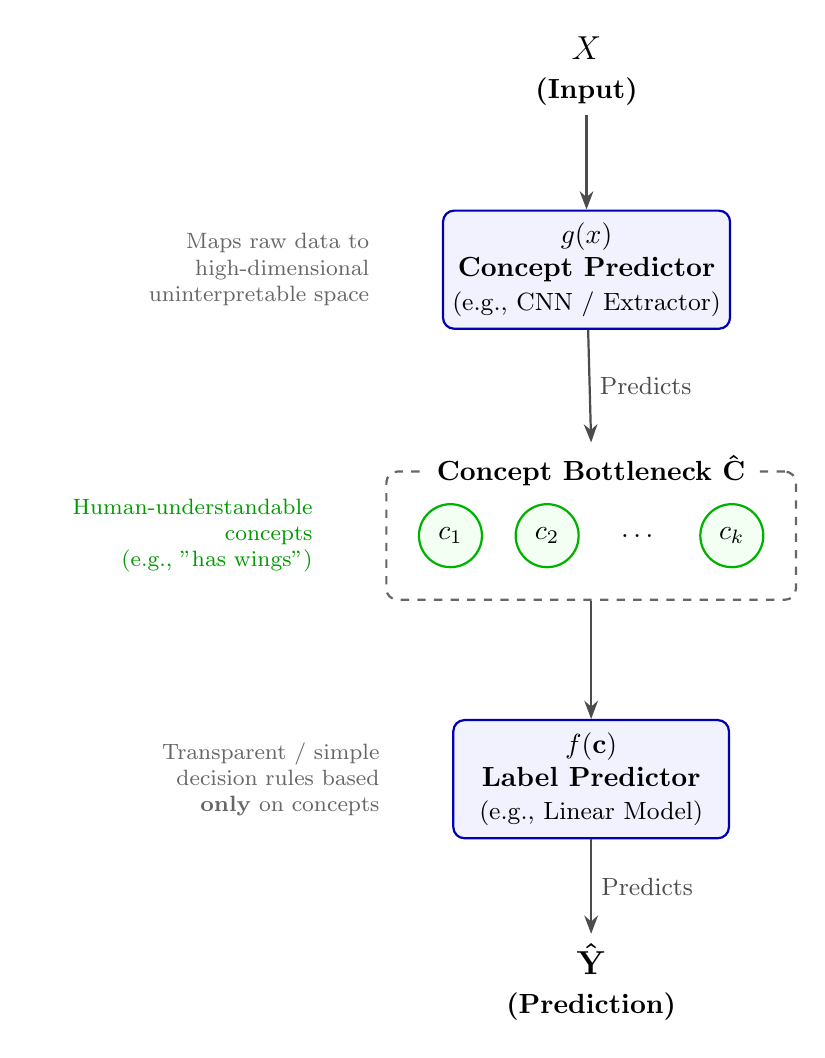
\begin{tikzpicture}[
    >=Stealth,
    % Styles
    box/.style={draw=blue!70!black, rectangle, rounded corners, align=center, minimum height=1.5cm, minimum width=3.5cm, fill=blue!5, thick},
    concept/.style={draw=green!70!black, circle, align=center, minimum size=0.8cm, fill=green!5, thick},
    io/.style={align=center, font=\large\bfseries}
    ]

    % 1. Input
    \node (input) [io] {$X$ \\ \normalsize (Input)};

    % 2. Concept Predictor g(x)
    \node (g) [box, below=1.2cm of input] {$g(x)$ \\ \textbf{Concept Predictor} \\ \small (e.g., CNN / Extractor)};

    % 3. Concept Bottleneck
    % Increased spacing below g(x) to give the arrow and 'Predicts' text room to breathe
    \node (c2) [concept, below=2.2cm of g, xshift=-0.5cm] {$c_2$};
    \node (c1) [concept, left=0.4cm of c2] {$c_1$};
    \node (cdots) [right=0.4cm of c2] {$\dots$};
    \node (ck) [concept, right=0.4cm of cdots] {$c_k$};

    % Group the concepts inside a dashed box
    \node[draw=black!60, rectangle, dashed, rounded corners, fit=(c1) (c2) (cdots) (ck), inner sep=0.4cm, thick] (c_box) {};

    % Place the label ON the top border (acting as a title between the arrow and the concepts)
    \node (c_label) [fill=white, font=\bfseries, inner sep=0.15cm] at (c_box.north) {Concept Bottleneck $\mathbf{\hat C}$};

    % 4. Label Predictor f(c)
    \node (f) [box, below=1.5cm of c_box] {$f(\mathbf{c})$ \\ \textbf{Label Predictor} \\ \small (e.g., Linear Model)};

    % 5. Output
    \node (output) [io, below=1.2cm of f] {$\mathbf{\hat Y}$ \\ \normalsize (Prediction)};

    % Connections / Arrows
    \draw[->, thick, draw=black!70] (input) -- (g);
    % Arrow points directly to the top of the new label
    \draw[->, thick, draw=black!70] (g) -- (c_label.north) node[midway, right, font=\small, text=black!70] {Predicts};
    \draw[->, thick, draw=black!70] (c_box.south) -- (f.north);
    \draw[->, thick, draw=black!70] (f.south) -- (output.north) node[midway, right, font=\small, text=black!70] {Predicts};

    % Descriptive Annotations (Anchored to the left)
    \node[left=0.8cm of g, text width=3.2cm, align=right, font=\footnotesize, color=gray!80!black] {Maps raw data to \\ high-dimensional \\ uninterpretable space};
    \node[left=0.8cm of c_box, text width=3.5cm, align=right, font=\footnotesize, color=green!60!black] {Human-understandable \\ concepts \\ (e.g., "has wings")};
    \node[left=0.8cm of f, text width=3.2cm, align=right, font=\footnotesize, color=gray!80!black] {Transparent / simple \\ decision rules based \\ \textbf{only} on concepts};
\end{tikzpicture}
\caption{Architecture of a Concept Bottleneck Model (CBM). The model maps a raw inputs $\mathbf{x}$ to an interpretable intermediate concept space $\mathbf{\hat c}$ before masking the final prediction $\mathbf{\hat y}$.}
\label{fig:cbm_architecture}
\end{figure}

\section{Information Leakage}   
For these types of models, it may often be unrealistic to assume that we will have access to concepts which fully capture the 
relationship between the inputs and targets. Several recent papers have studied the problem of information leakage in these types 
of models based on the previous assumption. This information leakage is usually observed in CBMs trained sequentially or jointly 
\cite{margeloiu2021conceptbottleneckmodelslearn, mahinpei2021promisespitfallsblackboxconcept}, and it appears when the intermediate 
representations encode information that is not present in the concepts $c$, which contains information to predict the final target 
rather than only focusing on getting the concept correct. This leakage has a negative impact on the interpretability and intervenability 
of the model. A CBM model with information leakage may be unsafe for critical decision-making applications, such as clinical scenarios. 
\cite{parisini2026leakageinterpretabilityconceptbasedmodels} We can identify two main types of leakage:   
\begin{itemize}
    \item \textbf{Concept-task leakage}: additional information about the task is stored in the learnt concepts. If concept-task 
    leakage is present, then the learned concept-task mutual information (MI) will be higher than ground-truth concept-task MI. 
    \item \textbf{Interconcept leakage}: additional information about the other concepts is stored in each learned concept. Learned 
    concepts are more predictive of the value of the other learned concepts, resulting in a learned interconcept MI being higher 
    than the ground-truth. 
\end{itemize} 
Several measures of leakage have been proposed in the literature, but none of them has successfully integrated the information-theoretic 
nature of leakage in these types of models. 
\begin{itemize}
    \item \textbf{Concept Performance Metrics}: these are the metrics that indicate the quality of the concept learning, such as for example 
    concept accuracy, precision, recall, F1 score and AUC. These metrics are not sensitive to leakage. Two models can have similar concept 
    performance but have different degrees of information leakage. Concept AUC has more sensitivity in this problem since it contains more 
    information about the concept distribution. 
    \item \textbf{Oracle Impurity Score (OIS)}: this metric was defined in \cite{Espinosa_Zarlenga_2023} to capture leakage. The idea is to 
    train $k(k-1)$ additional simple MLP $\psi_{i,j}$, whose objective is to predict the value of the ground-truth concept $j$ from the 
    learnt representation of concept $i$. This will create the Purity Matrix, defined as $\pi(\hat c, c) = AUC(\psi_{i,j}(\hat c_i), c_j)$. 
    The $(i,j)$-th entry contains the AUC when predicting the ground truth value of concept $j$ given the $i$-th concept representation. 
    The OIS metric is the average difference between the predictivities of learnt and ground truth concepts over pairs of concepts, defined 
    as $$OIS(\hat c, c) = \frac{2}{k} ||\pi(\hat c, c) - \pi(c,c)||_F$$, where the Frobenius norm ensures $0\leq OIS\leq 1$. The value of 
    1 represents a complete misalignment; the $i$-th concept can predict all other concepts except its corresponding one. A value of 0 
    represents a perfect alignment; the $i$-th concept does not encode any unnecessary information for predicting concept $i$. A limitation 
    is the stochasticity of the metric, which involves training neural networks, which is very variable when we evaluate the model several 
    times at test time. 
    \item \textbf{Niche Impurity Score (NIS)}: 
    \item \textbf{Intervention}: the intervention of the predicted concepts with the ground-truth values can be used to evaluate the 
    interpretability and the leakage. A task accuracy that decreases after intervention indicates that the task head expects extra information 
    that is not present in the ground-truth concepts. Models with higher leakage have worse intervention performance. This metric is unable 
    to distinguish between interconcept and concept-task leakage; also, when we have a large number of concepts, the computation is very expensive. 
\end{itemize}




\section{Recent CBMs}  

Concept Embedding Models \cite{zarlenga2022conceptembeddingmodelsaccuracyexplainability} \\
\\
Energy-based Concept Bottleneck Models (ECBMs) \cite{xu2024energybasedconceptbottleneckmodels}

\section{Concept Bottleneck Generative Models}


All the previous models presented in this document are focused on classification or regression problems, which are the original implementations 
of concept bottleneck models. The next step is to combine this idea with generative models to develop a method for interpreting and intervening 
in them, called Concept Bottleneck Generative Models (CBGMs)\cite{ismail2024concept}. This method allows us to steer the generative model, since 
we can change the concept of the image while preserving the image quality, and understand the model by identifying the important concepts that 
are responsible for the output. \\
The general idea is to insert a concept bottleneck (CB) layer into a generative model, which is divided in two parts: the pre-concept bottleneck 
part and the post-concept bottleneck part. The partition depends on the generative model we use (GANs, VAEs, Diffusion). The authors decided to 
use the Concept Embedding framework \cite{zarlenga2022conceptembeddingmodelsaccuracyexplainability} for the concept bottleneck layer and also 
argue that it is unrealistic to expect that the pre-defined human concepts are complete, so they also added a set of unknown concepts that might 
also be required for generation. \\
Each concept is represented with two embeddings: $w_i^+,w_i^- \in \mathbb{R}^m$ representing the active and inactive concept states, respectively. 
The output of the pre-concept bottleneck part of the model, the embedding $h$, is fed into several context networks $\phi$ that map $h$ to the 
two embeddings per concept. Then, a network $\Psi$ is trained to predict the probability of concept $c_i$ from the joint embedding space, 
$\hat c_i = \Psi_i([w_i^+, w_i^-]^T)\in[0,1]$. The final context embedding $w_i$ is defined as a weighted mixture of the two embeddings as 
$w_i=(\hat c_i w_i^+ + (1-\hat c_i)w_i^-)$. All the $k$ concept embeddings are concatenated to obtain the final vector that is fed to the 
post-concept network. For the intervention, we simply have to modify the concept probability $\hat c_i$ to $\bar c_i$ in the weighted mixture of 
$w_i$. A visualization of the concept layer is shown in Figure \ref{fig:cgbm_architecture}.
\begin{figure}
    \centering
    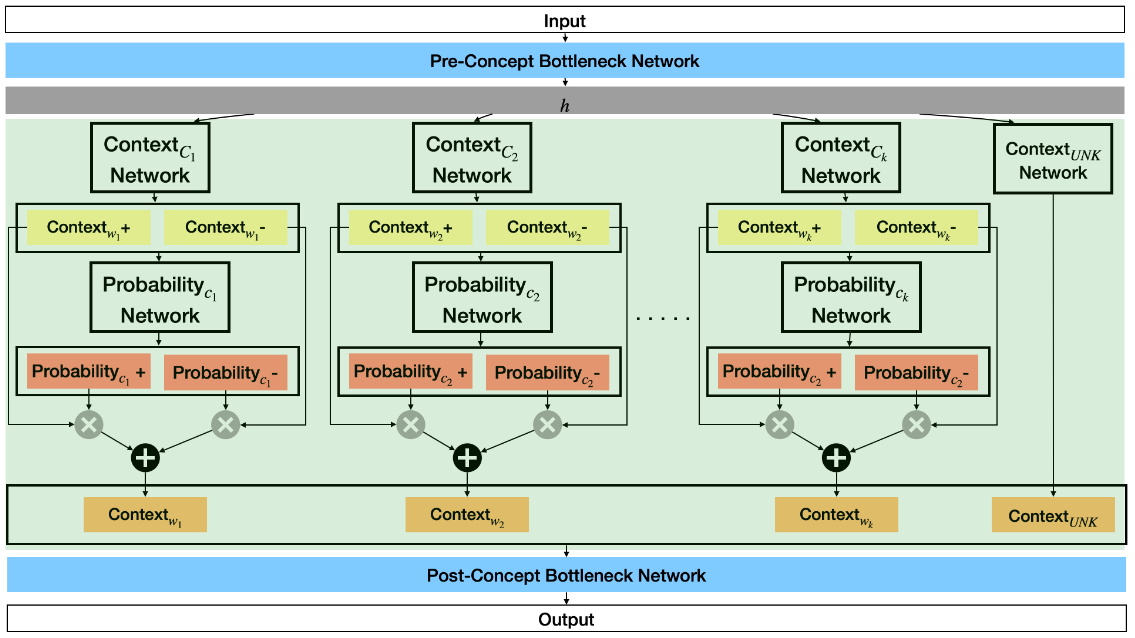
\includegraphics[width=0.9\linewidth]{gfx/cbm/cbgm.png}
    \caption{Architecture of the concept layer in the Concept Bottleneck Generative Model (CBGM) for a generic generative model.}
    \label{fig:cgbm_architecture}
\end{figure}
The loss function is defined as $$\mathcal{L} = \mathcal{L}_{task} + \alpha\mathcal{L}_{con} + \beta\mathcal{L}_{orth},$$ where $\alpha$ and 
$\beta$ are hyperparameters that control the importance of the concept and orthogonality loss, respectively. As we can see, the loss consists 
of three parts: 
\begin{itemize}
    \item \textbf{Task Loss}: the base objective function of the generative model family. 
    \item \textbf{Concept Loss}: is the binary cross-entropy loss between the predicted and real concept probabilities. 
    \item \textbf{Concept Orthogonality Loss}: encourage the unknown concepts to be orthogonal to the outputs of each concept network using an orthogonality constraint defined as: $$\mathcal{L}_{orth} = \sum_{f\in B}\frac{\sum_{i=1}^{i=k}|\langle w_i, w_{k+1} \rangle|}{\sum_{i=1}^{i=k}1},$$ where $\langle \cdot, \cdot \rangle$ is the cosine similarity and $j$ denotes each sample in the mini-batch of size $B$. 
\end{itemize} 
One of the main limitation of the previous method is that the generative model needs to be trained from scratch with the new concept bottleneck 
layer and using a dataset with ground-truth concept annotations. To build a more efficient and scalable method, we can use post-hoc generative 
concept bottleneck models \cite{kulkarni2025interpretablegenerativemodelsposthoc}, which can transform any pre-trained generative model into a 
interpretable one with concept bottleneck layer.  \\
Based on the setup of the previous method, where we divided the generative model in two parts ($g = g_2 \circ g_1$, $\mathbf{z}$ initial noise, 
$\mathbf{x}$ generated sample where $\mathbf{x} = g_2(g_1(\mathbf{z})))$, the idea is to include a concept bottleneck autoencoder. The latent 
space of the autoencoder is the concept prediction $\mathbf{c} = E(g_1(\mathbf{z}))$. This concept prediction is defined using the concept embedding 
framework and also includes a set of unknown concepts to complement the human-defined concepts. Then, the decoder $D$ reconstructs the features from 
the fist part of the generative model ($g_1$) based on the concept prediction $\mathbf{c}$, $\mathbf{w'}=D(\mathbf{c})$, where $\mathbf{w}=g_1(\mathbf{z})$
are the original features. Now we can generate samples from the original image features $\mathbf{w}$ as well as from the reconstructed features $\mathbf{w'}$, 
defined as $\mathbf{x}' = g_2(\mathbf{w'}) = g_2(D \circ E(\mathbf{w}))$.
\begin{figure}
    \centering
    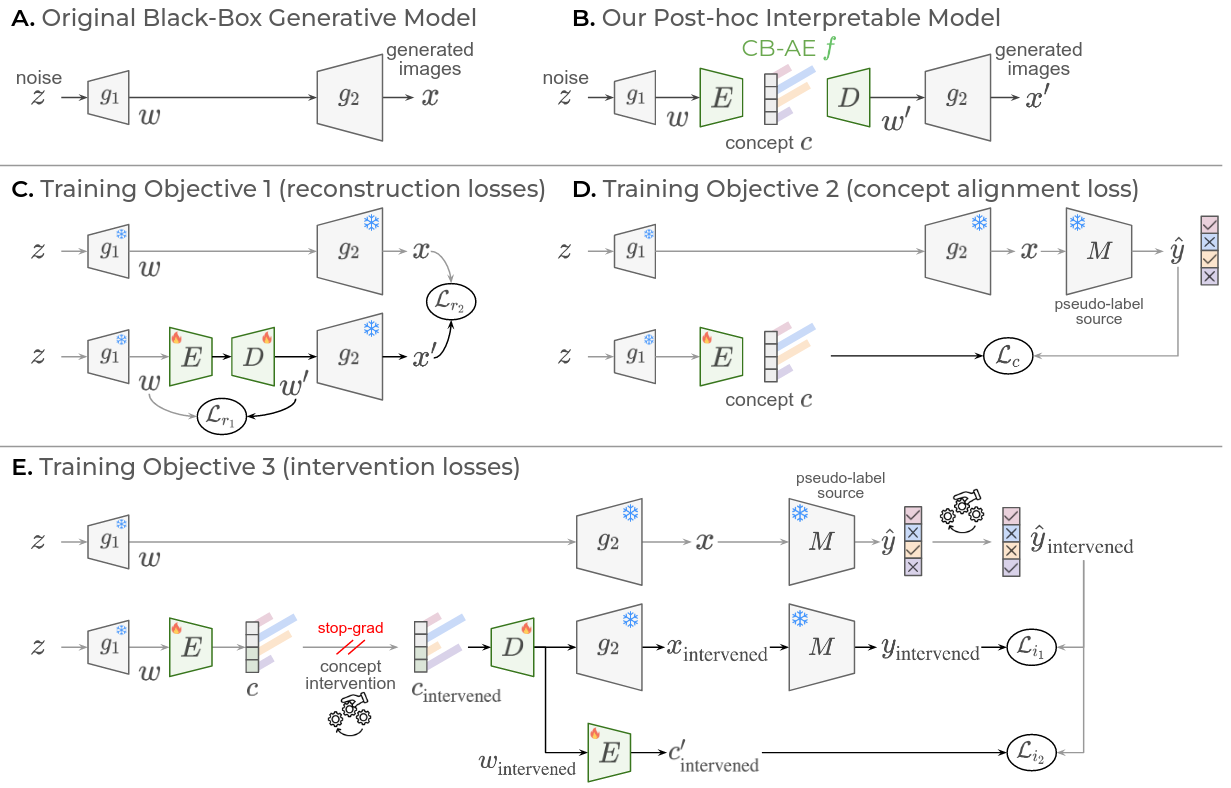
\includegraphics[width=0.9\linewidth]{gfx/cbm/post-hoc_cbgm.png}
    \caption{Architecture of the Post-hoc Concept Bottleneck Generative Model where the different loss functions are illustrated.}
    \label{fig:post_cgbm_architecture}
\end{figure}
For the training of this model, where the generative model is keep frozen, the authors defined three different objective functions based on the different desired goals: 
\begin{itemize}
    \item \textbf{Reconstruction Losses}: we sample $\mathbf{w}$ from the first part of the generative model and use it to generate the original image $\mathbf{x}$. The,
    we introduce $\mathbf{w}$ in the autoencoder to get the reconstructed features $\mathbf{w}'$, which is used to generate the reconstructed image $\mathbf{x}'$. The 
    reconstruction losses are defined as the distance between the original and reconstructed features and images, respectively. The definition is the following: 
    \begin{equation}
        \min_{E,D} \left[ \mathcal{L}_{r_1}(\mathbf{w}, \mathbf{w}') + \mathcal{L}_{r_2}(\mathbf{x}, \mathbf{x}') \right].
    \end{equation}
    \item \textbf{Concept Alignment Loss}: first we have to obtain the pseudo-labels $\mathbf{\hat y} = M(\mathbf{x})$ from a generated image $\mathbf{x}$. This model $M$ can be
    a supervised model or a zero-shot model, such as CLIP. Then, we can obtain the concept prediction $\mathbf{c} = E(g_1(\mathbf{z}))$ and use it to generate the image $\mathbf{x}'$. 
    We can also obtain the pseudo-labels $\mathbf{\hat y'} = M(\mathbf{x}')$ from the generated image. The concept alignment loss is defined as the distance between the pseudo-labels 
    of the original and the predicted concepts. The definition is the following:
    \begin{equation}
        \min_{E} \mathcal{L}_{c}(\mathbf{\hat y}, \mathbf{c}).
    \end{equation}
    \item \textbf{Intervention Losses}: they added a third loss to encourage the steerability of the model, which is an important property of CBMs. The idea is to encourage the decoder 
    $D$ to produce realistic $\mathbf{w'}$ when the concepts are modified. First, we have to select a concept $i$ to intervene by swaaping the logits in the latent concept space to obtain the 
    $\mathbf{c}_{int}$. With the intervened concepts, we can reconstruct the intervened features $\mathbf{w}_{int}$ and the intervened image $\mathbf{x}_{int}$, and using the pseudo-labeler, we can 
    get the concept prediction $\mathbf{y}_{int} = M(\mathbf{x}_{int})$. The final step is to intervene the pseudo-label of the original image by changing only the concept $i$ and get 
    $\mathbf{\hat y}_{int}$. The intervention loss is defined as the distance between the intervened pseudo-labels, which encourages the model to generate images that reflect the concept changes. 
    The definition is the following: 
    \begin{equation}
        \min_{E,D} \mathcal{L}_{i_1}(\mathbf{\hat y}_{int}, \mathbf{y}_{int}).
    \end{equation}
    Also, to improve consistency, they pass the intervened features $\mathbf{w}_{int}$ through the encoder to get the concept predction $\mathbf{c'}_{int}$ and apply cross-entropy loss defined as:
    \begin{equation}
        \min_{E, D} \mathcal{L}_{i_2}(\mathbf{\hat y}_{int}, \mathbf{c'}_{int}).
    \end{equation}
\end{itemize}
The next step is the method called Concept Bottlenecks on Energy Landscapes (CoBEla) \cite{kim2026cobelasteeringtransparentgeneration}, which presents a decoder-free and 
energy-based framework that use a pre-trained frozen generative model. Assume we have the same setup as before, with a generative model divided in two parts and a pseudo-labeler. 
They perturb the intermediate features using the DDPM cosine scheduler to get $\mathbf{w}_t$. For each concept $k$, they define an energy network $E_{\theta}$ that takes as input 
the perturbed features $\mathbf{w}_t$ and the concept $c_k$, which is a learnable concept embedding. The encoder outputs two logits and it is defined as two conditional residual blocks with 
FiLM conditioning \cite{perez2017filmvisualreasoninggeneral}. The concept score is defined as the positive-class probability, which leads to the definition of the interpretable bottleneck score vector
$\mathbf{s} = [s_1, s_2, \ldots, s_K]$. Then, the logits are converted into scalars to represent the energy for each concept, where the aggregation of per-concept energies is defined as 
$\mathcal{E}_{\theta}(\mathbf{w}_t)$, which is used in the score matching loss (defined in Section -- and Equation --) as the noise prediction of the energy-based model. As a complementary loss, 
we have the concept loss that compare the per-concept logits with the pseudo-labels. The total objective is defined as 
\begin{equation}
    \mathcal{L}(\theta) = \lambda_1\mathcal{L}_{score} + \lambda_2\mathcal{L}_{concept}.
\end{equation} 
The visualization of the framework is shown in Figure \ref{fig:cobela_architecture}. 
\begin{figure}
    \centering
    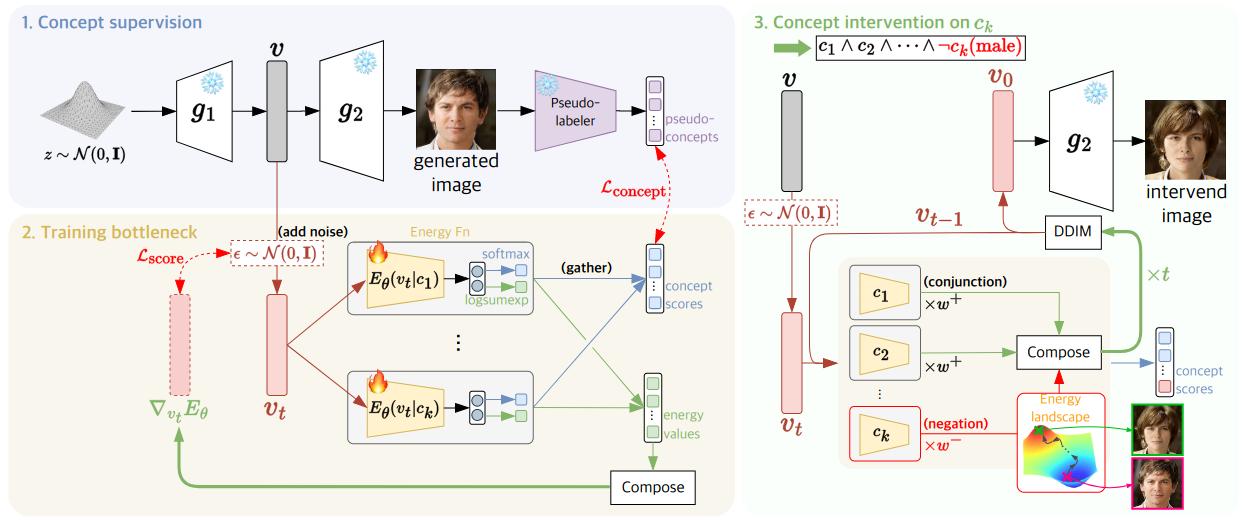
\includegraphics[width=0.9\linewidth]{gfx/cbm/cobela.png}
    \caption{Architecture of the CoBEla Model where the training and guided generation processes are illustrated.}
    \label{fig:cobela_architecture}
\end{figure}
In test time, we assign an intervention weight to each concept that yields to the final weighted energy defined as:
\begin{equation}
    \mathcal{E}_{\theta}(\mathbf{w}_t) = \sum_{k=1}^K \lambda_k E_{\theta}(\mathbf{w}_t, c_k).
\end{equation}
This model allows for the conjunction and negation of concepts, which is a very interesting property that allows for more complex interventions. They used the DDIM sampling method to obtain the final 
generated intermediate features using the weighted energy, which is then fed to the second part of the generative model to get the final generated image.


%*****************************************
%*****************************************
%*****************************************
%*****************************************
%*****************************************
\cleardoublepage
%\ctparttext{}
\part{Methods}
%************************************************
\chapter{Proposal}\label{ch:proposal}
%************************************************

Proposal.



%*****************************************
%*****************************************
%*****************************************
%*****************************************
%*****************************************
%************************************************
\chapter{Data}\label{ch:data}
%************************************************

In this section I want to introduce the different datasets that I have used during this part of my research and the possible 
future datasets that I plan to use in the remaining part of my thesis. In this initial part where I have focused on the 
implementation of some methods found in the literature along with some small experiments to have an intuition about the 
field, I have used a collection of small and well known in the literature datasets. These datasets are the following:
\begin{itemize}
    \item \textbf{MNIST} \cite{lecun1998mnist}: a dataset of handwritten digits with 60,000 training samples and 10,000 test samples, 
    where each sample is a 28x28 grayscale image of a digit from 0 to 9. 
    \item \textbf{Shapes2D} \cite{locatello2019challenging}: a dataset of 2D shapes with 737,280 samples, where each sample is a 64x64 
    RGB image of a shape (square, ellipse or heart) with different colors and sizes.
    \item \textbf{Shapes3D} \cite{locatello2019challenging}: a dataset of 3D shapes with 480,000 samples, where each sample is a 64x64 
    RGB image of a 3D shape (cube, sphere or cylinder) with different colors and sizes.
    \item \textbf{dSprites} \cite{dsprites17}: a dataset of 2D sprites with 737,280 samples, where each sample is a 64x64 grayscale image 
    of a sprite with different shapes, colors and positions. 
    \item \textbf{CelebA} \cite{liu2015faceattributes}: a dataset of celebrity faces with 202,599 samples, where each sample is a 178x218 
    RGB image of a celebrity face with different attributes (gender, age, hair color, etc.).
    \item \textbf{CelebA-HQ} \cite{karras2017progressive}: a dataset of high-quality celebrity faces with 30,000 samples, where each sample 
    is a 1024x1024 RGB image of a celebrity face with different attributes (gender, age, hair color, etc.).
\end{itemize}



%*****************************************
%*****************************************
%*****************************************
%*****************************************
%***************************************** 
\part{Experiments and Results} 
%************************************************
\chapter{Unconditional Flow Matching Model for X-Ray Images}\label{ch:exp1}
%************************************************

As discussed in the literature review, most recent techniques modify existing pre-trained generative models, often 
by adding extra components or introducing latent space disentanglement, to improve performance, interpretability, or compositionality  
without reducing the efficiency. However, these foundational models are generally trained on large, broad datasets rather than the 
medical data central to this thesis. To address this domain gap, I trained an unconditional flow matching model 
directly on a medical dataset, establishing a tailored pre-trained baseline for subsequent experiments. 
It is not intended to achieve SOTA performance, but rather to provide a baseline model to be used in the following experiments
to study disentanglement and compositionality in the medical domain. \\
\\
This study utilized the NIH-Chest-X-ray dataset (see Chapter \ref{ch:data} for more details) alongside the Representation Autoencoder 
(RAE) framework \cite{zheng2025diffusiontransformersrepresentationautoencoders}. Within this method, image latent representations are 
generated using a pre-trained visual model, specifically, a DINOv2-Base model configured with 4 register tokens 
\cite{oquab2024dinov2learningrobustvisual,darcet2024visiontransformersneedregisters}. The original RAE authors trained a decoder to 
construct an autoencoder from a large pre-trained visual model, yielding latents that offer richer semantic meaning and superior 
reconstruction quality compared to the SD-VAE latents typically used in state-of-the-art Stable Diffusion models. Subsequently, 
they trained a flow matching model on these RAE latents using a Diffusion Transformer (DiT), achieving good results but with a high 
computational cost because of the high-dimensional nature of the latents. To accommodate this problem, they also propose a modification 
of the DiT that incorporates architectural modifications inspired by Decoupled Diffusion Transformer (DDT) models, which 
prevent the need to scale the width across the entire backbone. When trained on ImageNet, this model achieved SOTA performance in both 
FID and IS metrics compared to other pixel and latent diffusion models. \\
\\
Because of the impressive generation quality of the model presented in the RAE paper and the quality and utility of the RAE latents, 
I decided to train a similar model on the NIH-Chest-X-ray dataset. I decided to train a DiT-XL (DINOv2-B) model insted of the improved 
DiT$^{DH}$-XL because I want to have a real bottleneck to perform further experiments. 

\begin{table}[ht]
    \centering
    \caption{Hyperparameter configuration used for training.}
    \label{tab:exp1_params}
    \renewcommand{\arraystretch}{1.25}
    \begin{tabular}{@{}llc@{}}
        \toprule
        \textbf{Category}       & \textbf{Hyperparameter}       & \textbf{Value}        \\
        \midrule
        \multirow{4}{*}{Optimization}
                                & Optimizer                     & AdamW                 \\
                                & Learning rate                 & $2 \times 10^{-4}$    \\
                                & Weight decay                  & $0.0$    \\
                                & Gradient clip norm            & $1.0$                 \\
        \midrule
        \multirow{3}{*}{Schedule}
                                & Warmup epochs                 & $40$             \\
                                & LR schedule                   & Linear      \\
                                & Final learning rate           & $2 \times 10^{-5}$    \\
        \midrule
        \multirow{4}{*}{Architecture}
                                & Input size                    & $16$                 \\
                                & Patch size                    & $1$                 \\
                                & In channels                   & $768$                 \\
                                & Hidden dimension              & $1152$                 \\
                                & Depth                         & $28$                  \\
                                & Attention heads               & $16$                   \\
                                & Dropout                       & $0.1$                 \\
        \midrule
        \multirow{3}{*}{Training}
                                & Batch size                    & $128$                 \\
                                & Mixed precision               & \texttt{float32}     \\
                                & EMA decay                     & $0.995$              \\
                                & Training epochs               & $450$                 \\
                                & Training steps                & $222$                 \\
        \bottomrule
    \end{tabular}
\end{table}


\begin{table}[ht]
    \centering
    \caption{Performance metrics of the DiT-XL (DINOv2-B) trained on the NIH-Chest-X-ray dataset.}
    \label{tab:exp1_results}
    \begin{tabular}{@{}lcccccc@{}}
        \toprule
        \textbf{Model}      & \textbf{Epochs}       & \#\textbf{Params}      & \textbf{FID}$\downarrow$      & \textbf{IS}$\uparrow$     & \textbf{Precision}$\uparrow$      & \textbf{Recall}$\uparrow$     \\
        \midrule
        DiT-XL   & --                    & --                    & --                            & --                        & --                    & --                    \\
        DiT$^{DH}$-XL   & --                    & --                    & --                            & --                        & --                    & --                    \\
        \bottomrule
    \end{tabular}
\end{table}
 


%*****************************************
%*****************************************
%*****************************************
%*****************************************
%***************************************** 
%************************************************
\chapter{Slot Attention with Concept Supervision in CelebA-HQ}\label{ch:exp2}
%************************************************

After the literature review about Slot Attention and other Object-Centric Learning methods, where all the explanations can be found in Section --, some connections with Concept Bottleneck Models (Section --) arise naturally. Both paradigms inherently seek to decompose complex, high-dimensional visual inputs into a discrete set of interpretable variables before performing downstream reasoning. In both frameworks, the architecture forces the model to route its decision-making process through a constrained intermediate layer—whether it is a set of permutation-invariant slots representing physical entities, or a vector of semantic concepts aligned with human logic. \\
\\
Despite this shared structural philosophy, there are fundamental differences in their objectives and learning signals. Object-Centric Learning methods like Slot Attention are traditionally unsupervised, relying on spatial competition and reconstruction objectives to discover emergent, perceptual groupings. In contrast, Concept Bottleneck Models are explicitly supervised, requiring ground-truth labels to map visual features directly to predefined, high-level semantics. Furthermore, while traditional CBMs often struggle to spatially ground their concepts within specific regions of an image, Slot Attention excels at isolating localized areas but lacks the guarantee that a discovered slot will align with a human-understandable trait. \\
\\
Recognizing both the complementary strengths and the distinct differences between these approaches, this section introduces an experiment that bridges the two. By applying explicit concept supervision to a Slot Attention module, we aim to spatially ground predefined facial attributes from the CelebA-HQ dataset directly into distinct visual slots. To ensure the slots can specialize entirely on these localized semantic traits, our architecture incorporates register tokens designed to independently capture and store extra global image context. 


\begin{figure}
    \centering
    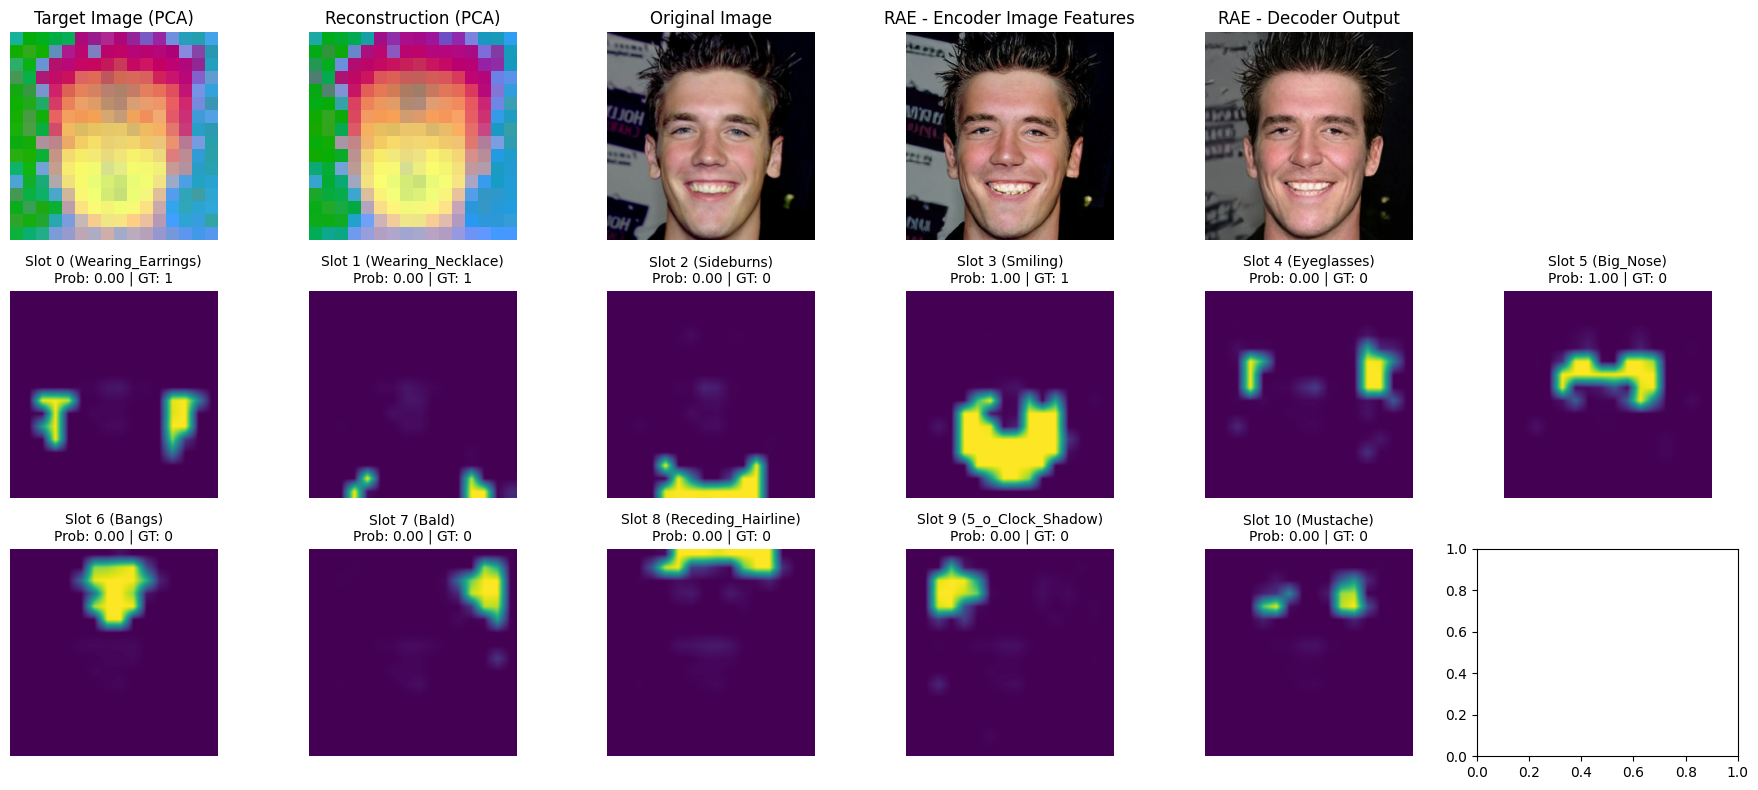
\includegraphics[width=\linewidth]{gfx/exp2/supervised_sa_1.png}
    \caption{Caption}
    \label{fig:supervised_sa_1}
\end{figure}
\begin{figure}
    \centering
    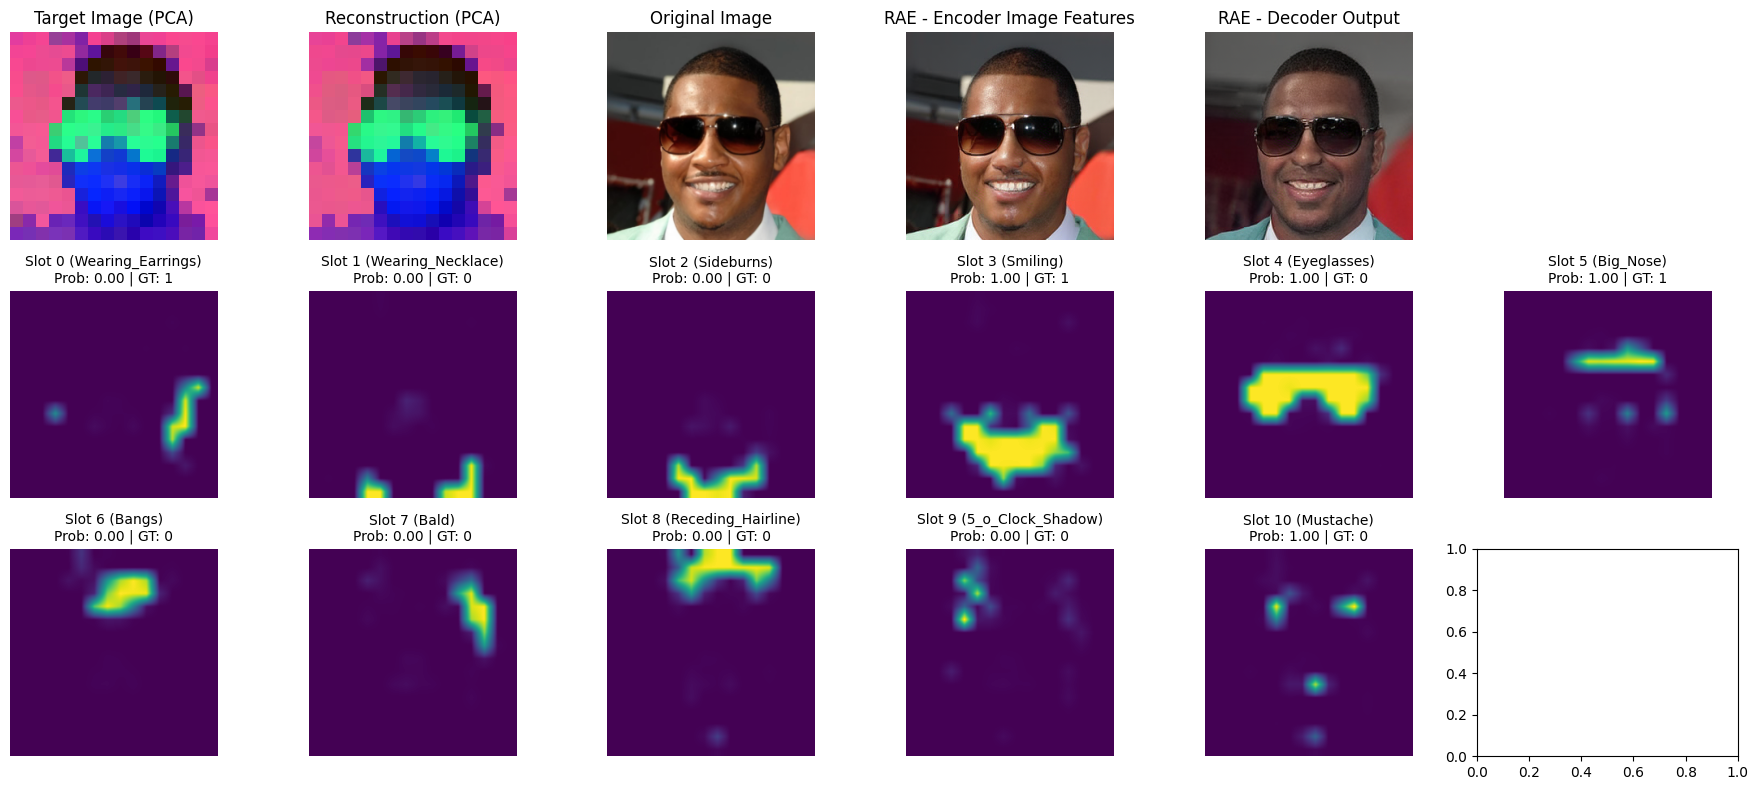
\includegraphics[width=\linewidth]{gfx/exp2/supervised_sa_2.png}
    \caption{Caption}
    \label{fig:supervised_sa_2}
\end{figure}
\begin{figure}
    \centering
    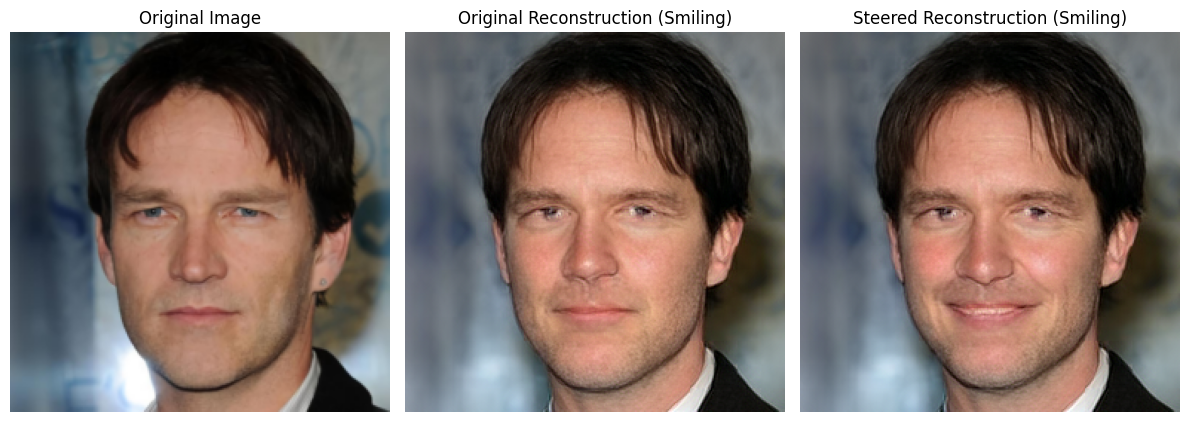
\includegraphics[width=\linewidth]{gfx/exp2/steer_smiling.png}
    \caption{Caption}
    \label{fig:steer}
\end{figure}





%*****************************************
%*****************************************
%*****************************************
%*****************************************
%*****************************************
\part{Research Plan}
%************************************************
\chapter{Timeline}\label{ch:timeline}
%************************************************

In this chapter I want to update the timeline of my PhD based on the one presented in the initial Research Plan. The project can 
be organized in different stages, which can be the same as the ones presented previously. A Gantt chart showing the different stages 
and their expected duration is also included in Figure \ref{fig:timeline}. 
\begin{itemize}
    \item \textbf{Stage 1: Literature Review and Theoretical Foundations}. This stage will involve an in-depth review of the existing 
    literature on deep generative models (VAEs, Diffusion and Flow Matching), disentanglement representation learning, compositionality, 
    concept bottleneck models, and generative AI for the medical domain. I will also study the theoretical foundations of these 
    topics to identify gaps and opportunities for my research, the key challenges and research questions and define the quantitative and 
    qualitative metrics that I will use to evaluate the performance of my proposed methods. \\
    This stage was planned to be completed in the first 6 months of the PhD, and I have already made significant progress in this area, having 
    reviewed a large number of relevant papers and identified key research questions and challenges that I will address in my research. In the 
    review timeline I have extended the review of the literature to the Q1 of the second year of the PhD, as I will continue to review new papers and 
    developments in the field throughout the duration of the project. 
    \item \textbf{Stage 2: Preliminary experiments}. In this stage, I will conduct preliminary experiments to explore the capabilities 
    and limitations of existing models in terms of disentanglement and compositionality. This will help me to define some baseline models 
    and metrics for evaluating the performance of my proposed methods. This include the reproduction of some key generative models like VAEs,
    Diffusion and Flow Matching, and the implementation of some disentanglement and compositionality metrics. \\
    This stage was planned to be completed between the first 6 and 12 months of the PhD. In the new timeline I have updated it to be between the 
    Q4 of the first year and the Q4 of the second year, with a natural overlap with the previous stage, since I found that implementing and experimenting with the models is a 
    great way to deepen my understanding of the literature and identify gaps and challenges. I have already started conducting several 
    implementations of key models and metrics, where some results were presented in the experiments section.  
    \item \textbf{Stage 3: Method Development and Architectural Innovation}. In this stage, I will develop new methods and architectures for 
    deep generative models that aim to achieve better disentanglement, compositionality, and controllability. This will involve 
    designing novel model architectures, training algorithms, and evaluation metrics to assess the performance of the proposed methods. The idea 
    is to implement modification and extensions of the generative models to enhance their capabilities. \\
    This stage was planned to be completed between the first 12 and 24 months of the PhD. In the new timeline I have modified it to be between the 
    Q3 of the second year and the Q2 of the third year, with a natural overlap with the previous stage, since the insights gained from the preliminary experiments will inform 
    the development of the new methods and architectures. I have already started to develop some preliminary ideas for new methods and architectures, 
    and I plan to continue refining and testing these ideas in the coming months. 
    \item \textbf{Stage 4: Application to the Medical Domain}. In this stage, I will apply the developed methods to the medical domain, 
    specifically focusing on the analysis of medical images focusing on domain-specific challenges like resolution, structure preservation, and clinical 
    realism. Collaborations with medical experts or institutions may be established to assess practical viability and gather expert feedback. Ethical, 
    legal, and data governance considerations will also be reviewed during this phase. In this stage I  will start to work with curated medical image datasets,
    and I will evaluate the performance of the proposed methods in terms of their ability to generate high-quality, clinically relevant images, and to provide 
    insights into the underlying data. \\
    This stage was planned to be completed between the 24 to 30 months of the PhD. In the new timeline I have modified it to be done between the Q2 
    of the third year and the Q1 of the fourth year, with some overlap with the previous stage, since the development of the new methods and architectures 
    will be informed by the specific challenges and requirements of the medical domain. 
    \item \textbf{Stage 5: Evaluation, Validation, and Writing}. In this final stage, I will conduct a comprehensive evaluation of the proposed methods, 
    including both quantitative and qualitative assessments. I will also validate the results through collaborations with domain experts and 
    prepare the findings for publication in peer-reviewed journals and conferences. Additionally, I will write the final thesis document, 
    summarizing the research contributions and outlining future directions for further research in this area. \\
    This stage is planned to be done during the last year of the PhD, between the Q2 and Q4 of the fourth year, with some overlap with the previous stage, 
    since the evaluation and validation of the proposed methods will be an ongoing process throughout the development and application stages. 
\end{itemize}

\begin{figure}[htbp]
    \centering
    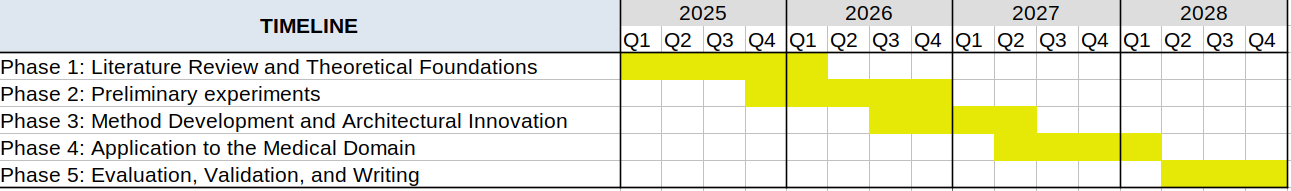
\includegraphics[width=\textwidth]{gfx/timeline/Timeline.png}
    \caption{Updated timeline of the PhD project, showing the different stages and their expected duration.}
    \label{fig:timeline}
\end{figure}


%*****************************************
%*****************************************
%*****************************************
%*****************************************
%*****************************************
%************************************************
\chapter{Data Management Plan}\label{ch:DataPlan}
%************************************************

This project relies entirely on pre-existing, curated, and de-identified datasets. 
No new primary data collection involving human subjects will be conducted. The data 
management strategy is structured in three progressive phases, transitioning from 
general-purpose computer vision datasets to restricted-access clinical datasets. \\
\\
The research will utilize the following datasets, categorized by project phase: 
\begin{itemize}
    \item \textbf{Phase 1: Prototyping and Baseline Implementation}: Initial architectural 
    development, debugging, and proof-of-concept experiments for disentangled generation 
    and compositionallity analysis will be conducted using well-known, publicly available 
    datasets. These include MNIST, Shapes3D, and CelebA. See Chapter \ref{ch:data} for a 
    detailed list and description of the datasets. These datasets are open-access and 
    require no special data use agreements. 
    \item \textbf{Phase 2: Medical Domain Adaptation}: To transition the generative models to the medical domain, publicly available medical imaging datasets will be utilized. While initial experiments will leverage established repositories like the NIH Chest X-ray and CheXpert datasets, this research is not restricted to radiography. The proposed methods are designed to be adaptable across diverse medical imaging modalities (e.g., MRI, CT, or histopathology). These datasets are fully de-identified and openly available for research purposes, providing a safe and ethical environment to test the models on complex anatomical structures and a wide variety of pathologies. A detailed description of these datasets can be found in Chapter \ref{ch:data}. 
    \item \textbf{Phase 3: Advanced Clinical Application}: For the final evaluation of 
    compositional generation and clinical realism, the project will utilize the MIMIC-CXR dataset. 
    This is a large, restricted-access database of chest radiographs. Access to the MIMIC-CXR 
    dataset has been formally granted via PhysioNet. I have completed the required credentialing 
    (e.g., CITI training on Data or Specimens Only Research) and signed the Data Use Agreement (DUA). 
    No attempts will be made to re-identify any patients. The original restricted data will not 
    be copied to unauthorized personal devices, and access will be limited solely to credentialed 
    researchers involved directly in this project. 
\end{itemize} 
All datasets will be securely stored at the Barcelona Supercomputing Center (BSC - MareNostrum 5) 
and on password-protected, encrypted local workstations used for prototyping. Throughout the project, 
the generative models will produce purely synthetic medical data (e.g., artificial radiographs 
and corresponding segmentation masks or labels). This synthetic data contains no real patient 
information and poses no privacy risks. Derived data, such as model weights, evaluation metrics, 
and latent embeddings, will also be generated and stored securely on the BSC infrastructure. 


%*****************************************
%*****************************************
%*****************************************
%*****************************************
%*****************************************
%************************************************
\chapter{Training Plan}\label{ch:TrainingPlan}
%************************************************

I will engage in a comprehensive training plan designed to strengthen my theoretical foundation, enhance my technical proficiency, and foster integration within the broader research community. As training activities are completed, they will be properly documented and recorded in the Doctoral Student Activity Document (DAD). This record will serve as a living document, continually updated throughout my doctoral studies. \\
\\
Throughout my PhD, I will participate in transversal training provided by the Doctoral School, logging these activities in DRAC to maintain my DAD. Specifically, I plan to undertake coursework related to open science and citizen science beginning in my second year, continuing into the third and fourth years. Additionally, I will cultivate essential soft skills—such as communication, leadership, and project management—through workshops, seminars, and courses offered by both the Doctoral School and the Barcelona Supercomputing Center (BSC). I will also actively attend conferences and workshops in the fields of deep generative models and medical imaging to network with peers and exchange novel ideas. \\
\\
My specialized training is already underway. In the summer of my first year, I attended the "MLx Representation Learning \& Generative AI" summer school at the University of Oxford. This program provided a comprehensive overview of state-of-the-art techniques, led by speakers at the forefront of the field. For the summer of my second year, I plan to attend the Probabilistic AI Summer School in Lithuania, which focuses on variational inference, diffusion models, and related topics. In the subsequent years of my PhD, I will continue to participate in relevant summer schools and conferences to stay abreast of emerging trends and expand my professional network.


%*****************************************
%*****************************************
%*****************************************
%*****************************************
%*****************************************
%\include{Chapters/Chapter02}
%\addtocontents{toc}{\protect\clearpage} % <--- just debug stuff, ignore
%\include{Chapters/Chapter03}
%\include{multiToC} % <--- just debug stuff, ignore for your documents
% ********************************************************************
% Backmatter
%*******************************************************
%\appendix
%\renewcommand{\thechapter}{\alph{chapter}}
%\cleardoublepage
%\part{Appendix}
%\include{Chapters/Chapter0A}
%********************************************************************
% Other Stuff in the Back
%*******************************************************
\cleardoublepage\include{FrontBackmatter/Bibliography}
%\cleardoublepage\include{FrontBackmatter/Declaration}
%\cleardoublepage\include{FrontBackmatter/Colophon}
% ********************************************************************
% Game Over: Restore, Restart, or Quit?
%*******************************************************
\end{document}
% ********************************************************************
